\documentclass[pdftex]{beamer}
%\documentclass[notes=show]{beamer}
%\documentclass[xcolor=dvipsnames]{beamer}
\usepackage{graphicx}
\usepackage{amssymb}
\usepackage{latexsym}
\usepackage{amsfonts}
\usepackage{amsmath}
\usepackage[absolute,overlay]{textpos}
\usepackage[english]{babel}
\usepackage[latin1]{inputenc}
%\usepackage{times}
\usepackage[T1]{fontenc}
\usepackage{tabularx}
\newcolumntype{Y}{>{\small\raggedright\arraybackslash}X}
\usepackage{graphicx}
\usepackage{bigstrut}
\usepackage{bbm}
\usepackage{mathrsfs}
\usepackage{epsfig}
\usepackage{array}
\usepackage{comment}

\mode<presentation> {
%\usetheme[left,width=1.7cm]{Berkeley}
%\usetheme{default}
\usetheme{Boadilla}
  \usecolortheme[RGB={103,102,204}]{structure}
%\usecolortheme{dove}
  \useoutertheme{infolines}
  \setbeamercovered{transparent}
 }

%\renewcommand{\familydefault}{cmss}
%\renewcommand{\mathrm}{\mathsf}
%\renewcommand{\textrm}{\textsf}
\usefonttheme{serif}
\newcommand{\X}{{\mathbf{X}}}
\newcommand{\x}{{\mathbf{x}}}
\newcommand{\E}{\mathsf{E}}
\newcommand{\V}{\mathsf{Var}}


    %%%%%%%%%%%%%%%%%%%%%%%%%%%%%%%%%%%%%%%%%%%%%%%%%%%%%%%%%%%%%%%%%%%%%%%%%%%%%%
    %         Neue Kommandos f�r fette Mathebuchstaben innerhalb von Formeln     %
    %%%%%%%%%%%%%%%%%%%%%%%%%%%%%%%%%%%%%%%%%%%%%%%%%%%%%%%%%%%%%%%%%%%%%%%%%%%%%%
    \newcommand{\bom}{\boldmath}
    \newcommand{\ubom}{\unboldmath}
    \newcommand{\mb}{\mathbf}

    \newcommand{\fmalpha}{\mbox{\bom${\alpha}$}}               %Fettes alpha
    \newcommand{\fmbeta}{\mbox{\bom${\beta}$}}                 %Fettes beta
    \newcommand{\fmgamma}{\mbox{\bom${\gamma}$}}               %Fettes gamma
    \newcommand{\fmdelta}{\mbox{\bom${\delta}$}}               %Fettes delta
    \newcommand{\fmepsilon}{\mbox{\bom${\epsilon}$}}           %Fettes epsilon
    \newcommand{\fmvarepsilon}{\mbox{\bom${\varepsilon}$}}     %Fettes varepsilon
    \newcommand{\fmzeta}{\mbox{\bom${\zeta}$}}                 %Fettes zeta
    \newcommand{\fmeta}{\mbox{\bom${\eta}$}}                   %Fettes eta
    \newcommand{\fmta}{\mbox{\bom${\theta}$}}                  %Fettes theta (ta)
    \newcommand{\fmvarta}{\mbox{\bom${\vartheta}$}}         	 %Fettes vartheta (ta)
    \newcommand{\fmiota}{\mbox{\bom${\iota}$}}                 %Fettes iota
    \newcommand{\fmkappa}{\mbox{\bom${\kappa}$}}               %Fettes kappa
    \newcommand{\fmla}{\mbox{\bom${\la}$}}                     %Fettes lambda (la)
    \newcommand{\fmmu}{\mbox{\bom${\mu}$}}                     %Fettes mu
    \newcommand{\fmnu}{\mbox{\bom${\nu}$}}                     %Fettes nu
    \newcommand{\fmxi}{\mbox{\bom${\xi}$}}                     %Fettes xi
    \newcommand{\fmo}{\mbox{\bom${\o}$}}                       %Fettes o
    \newcommand{\fmpi}{\mbox{\bom${\pi}$}}                     %Fettes pi
    \newcommand{\fmvarpi}{\mbox{\bom${\varpi}$}}               %Fettes varpi
    \newcommand{\fmrho}{\mbox{\bom${\rho}$}}                   %Fettes rho
    \newcommand{\fmvarrho}{\mbox{\bom${\varrho}$}}             %Fettes varrho
    \newcommand{\fmsigma}{\mbox{\bom${\sigma}$}}               %Fettes sigma
    \newcommand{\fmvarsigma}{\mbox{\bom${\varsigma}$}}         %Fettes varsigma
    \newcommand{\fmtau}{\mbox{\bom${\tau}$}}                   %Fettes tau
    \newcommand{\fmupsilon}{\mbox{\bom${\upsilon}$}}           %Fettes upsilon
    \newcommand{\fmphi}{\mbox{\bom${\phi}$}}                   %Fettes phi
    \newcommand{\fmvarphi}{\mbox{\bom${\varphi}$}}             %Fettes varphi
    \newcommand{\fmchi}{\mbox{\bom${\chi}$}}                   %Fettes chi
    \newcommand{\fmpsi}{\mbox{\bom${\psi}$}}                   %Fettes psi
    \newcommand{\fmomega}{\mbox{\bom${\omega}$}}               %Fettes omega
    \newcommand{\fmimath}{\mbox{\bom${\imath}$}}               %Fettes imath


\setbeamercolor{bibliography entry title}{fg=black}
\setbeamercolor{bibliography entry author}{fg=black}
\setbeamercolor{subsection in toc}{fg=structure}
\setbeamercolor{palette primary}{bg=structure, fg=white}
%\setbeamercolor{palette secondary}{bg=structure, fg=black}
%\setbeamercolor{palette tertiary}{bg=structure, fg=black}
\setbeamercolor{caption name}{fg=black} \setbeamersize{text margin
left=.8cm} \setbeamersize{text margin right=1cm}
\hypersetup{linkbordercolor={1 0 0}} \setbeamertemplate{navigation
symbols}{} \setbeamertemplate{headline}[default]

\setbeamertemplate{enumerate items}[default]

\newcounter{transfct}
\newcounter{begbs}
\newcounter{endbs}
\title[Instrumental Variables]{Econometrics 2 (Part 1)}

\author[Lychagin  \& Mu\c co]{Sergey Lychagin}
\institute[CEU]{Central European University}
\date{Winter 2020}

\AtBeginSection[] {
  \begin{frame}<handout:0>
    \frametitle{TOC}
    \tableofcontents[currentsection]
  \end{frame}
}

%\AtBeginSubsection[] {
%  \begin{frame}<beamer>
%   \frametitle{Outline}
%    \tableofcontents[currentsection,currentsubsection]
%  \end{frame}
%}

%\beamerdefaultoverlayspecification{<+->}

\begin{document}

\frame{\titlepage}


%slide 2

\begin{frame}
\frametitle{Motivation}
Early econometric research on 
\begin{itemize}
\item Simultaneous Equations Models
\item Measurement Error Bias
\end{itemize}
Today
\begin{itemize}
\item Omitted Variables Bias
\end{itemize}
\begin{itemize}
%
%\item 2 parts:
%      \begin{itemize}
%         \item Restricted model with constant coefficients (Potential outcomes are the same for everybody)\\
%         \item Unrestricted model with heterogenous potential outcomes
%      \end{itemize}
\item Applications:
         \begin{itemize}
           \item Effect of military service on earnings
           \item Effects of family size on female labor supply
           \item Returns to education
         \end{itemize}

\end{itemize}
\end{frame}


% slide 3


\begin{frame}
\frametitle{Omitted variables problem}
\begin{itemize}
\item Constant Effects Setup
\begin{eqnarray*}
	y_{si} &=& f_{i}\left(s\right) \\
  f_{i}\left(s\right) &=& \alpha+ \rho s+ \eta_{i} \\
  \eta_{i} &=& A_{i}^{'}\gamma+v_i,\;E[\eta_i|A_i] = A_i\gamma.
\end{eqnarray*}
\item $A_{i}$ are the only reason why $\eta_{i}$ and $s_{i}$ may be correlated: $s_i\amalg\eta_i |A_i$.
\item $\gamma$ --- population regression coefficients (not necessarily causal)


\[\begin{array}{cl}
    E\left[A_{i}v_{i}\right]&= 0\\
    E\left[s_{i}v_{i}\right]&= 0
    \end{array}
\]

\item If $A_{i}$ is observed:


\[\begin{array}{cl}
   Y_{i} =  \alpha+ \rho s_{i}+ A_{i}^{'}\gamma+v_{i} \Rightarrow $Long Regression$

    \end{array}
\]

\item Problems:
\begin {itemize}

   \item $A_{i}$ is unobserved, how can we estimate $\rho$?
\end{itemize}
\end{itemize}
\end{frame}



% slide 4

\begin{frame}
\frametitle{Instrumental Variable}
\begin{eqnarray*}
  Y_{i} = \alpha+ \rho s_{i}+\eta_{i}
\end{eqnarray*}
\begin{itemize}
\item Instrumental Variable
\begin {itemize}
    \item $z_{i}$ correlated with $s_{i}$, but uncorrelated with any other determinants of $Y_{i}$ (instrument relevance)
    \item $Cov\left(\eta_{i}, z_{i}\right)=0$, or $z_{i}$ uncorrelated with both $A_{i}$ and $v_{i}$ (instrument exogeneity)
\end {itemize}

\item \emph{Exclusion Restriction/Instrument exogeneity}:

\begin{eqnarray*}
  \rho=\frac{Cov\left(Y_{i}, z_{i}\right)}{Cov\left(s_{i}, z_{i}\right)} = \frac{Cov\left(Y_{i}, z_{i}\right)/V\left(z_{i}\right)}{Cov\left(s_{i}, z_{i}\right)/V\left(z_{i}\right)}
\end{eqnarray*}

\item Ratio of population regression of $Y_{i}$ on $z_{i}$ (\emph{reduced form}) and $s_{i}$ on $z_{i}$ (\emph{first stage}).

\end{itemize}
\end{frame}




% slide 5

\begin{frame}
\frametitle{Assumptions}
\begin{itemize}
\item 2 important assumptions:
   \begin {itemize}
    \item \emph{Relevance}: $z_{i}$ has an effect on $s_{i}$ (can be tested)
     \begin{eqnarray*}
            Cov\left(s_{i}, z_{i}\right)\neq 0
      \end{eqnarray*}
    \item \emph{Exogeneity/exclusion restriction:} $z_{i}$ affects $Y_{i}$ only via $s_{i}$:
     \begin{eqnarray*}
           Cov\left(\eta_{i}, z_{i}\right)= 0
      \end{eqnarray*}

\end{itemize}
\item How do we find Instrumental Variables?
     \begin {itemize}
     \item Institutional knowledge
     \item Ideas about the process determining $s_{i}$
\end {itemize}
\item Examples:
      \begin {itemize}
         \item Compulsory schooling law
          \item Schooling decision based on costs and benefits
          \item College proximity as determinant of schooling decision
\end {itemize}
\end {itemize}
\end{frame}


% slide 6

\begin{frame}
\frametitle{General model}
\begin{itemize}
\item Structural Equation
\begin{eqnarray*}
  Y_{i} = X_{i}' \alpha+ \rho s_{i}+\eta_{i}, \; E[\eta_i|X_i] = 0.
\end{eqnarray*}
    \begin {itemize}
       \item First Stage:
      \begin{eqnarray*}
           s_{i}= X_{i}^{'}\pi_{10}+ \pi_{11}z_{i}+ \xi_{1i}, \; E[\xi_{1i}|X_i, z_i] = 0
      \end{eqnarray*}
    \item Reduced Form:
        \begin{eqnarray*}
           Y_{i}= X_{i}^{'}\pi_{20}+ \pi_{21}z_{i}+ \xi_{2i}
      \end{eqnarray*}
\end {itemize}
\item $s_{i}$ and $Y_{i}$ are \emph{endogenous variables}. 	Fundamental issue: $\xi_{1i}$ correlates with $\eta_i$ (e.g. schooling and wage are driven by unobserved ability).
\item $z_{i}$ instrumental variable, conditionally  independent of $\eta_i$: $z_i\amalg \eta_i|X_i$.
\item $X_{i}$ --- controls

\end{itemize}
\end{frame}



%slide 7

\begin{frame}
\frametitle{Indirect Least Squares}


Covariate adjusted IV estimator:
\begin{eqnarray*}
  \rho=\frac{\pi_{21}}{\pi_{11}}=\frac{Cov\left(Y_{i}, \tilde{z_{i}}\right)}{Cov\left(s_{i},\tilde{ z_{i}}\right)}
\end{eqnarray*}
\begin {itemize}


\item $\tilde{z_{i}}$ residual from regressing $z_{i}$ on $x_{i}$ (regression anatomy)
\item Proof:
\begin{eqnarray*}
  Y_{i} &=& X_{i}' \alpha+ \rho s_{i}+\eta_{i}  \\
  Cov\left(Y_{i}, \tilde{z_{i}}\right)&=& \rho Cov\left(s_{i}, \tilde{z_{i}}\right)
\end{eqnarray*}
      \begin {itemize}
     \item $\tilde{z_{i}}$ uncorrelated with $X_{i}$ by construction.
     \item $\tilde{z_{i}}$ uncorrelated with $\eta_{i}$ by assumption (easy to check)
\end {itemize}
\end {itemize}

\end{frame}






% slide 8

\begin{frame}
\frametitle{Alternative Representation}


\[\begin{array}{cc}
   Y_{i} =  X_{i}' \alpha + \rho s_{i}+\eta_{i}

    \end{array}
\]

\begin{itemize}
\item Subsitute first stage

\begin{eqnarray*}
   Y_{i} &=& X_{i}' \alpha+ \rho\left[X_{i}'\pi_{10}+\pi_{11}z_{i}+ \xi_{1i}\right]+\eta_{i}\\
   Y_{i} &=&  X_{i}'\left[\alpha+ \rho \pi_{10}\right]+\rho \pi_{11}z_{i}+\left[\rho \xi_{1i}+\eta_{i}\right]
\end{eqnarray*}
   \item Reduced Form
\begin{eqnarray*}
   Y_{i}   &=&  X_{i}'\pi_{20}+\pi_{21}z_{i}+ \xi_{2i}
\end{eqnarray*}
\item Compare coefficients
 \begin{eqnarray*}
   \pi_{20}&=& \alpha+ \rho\pi_{10}\\
   \rho\pi_{11}&=& \pi_{21} \;\;\;\;\;\; \Rightarrow \rho=\frac{\pi_{21}}{\pi_{11}}\\
   \xi_{2i}&=& \rho\xi_{1i} + \eta_{i}\\
\end{eqnarray*}



\end{itemize}
\end{frame}


% slide 9

\begin{frame}
\frametitle{Two Stage Least Squares}

Re-write structural equation
\begin{eqnarray*}
 Y_{i} &=& X_{i}' \alpha+ \rho\underbrace{\left[X_{i}^{'}\pi_{10}+\pi_{11}z_{i}\right]}_{s^*_i}+\rho\xi_{1i}+\eta_{i} \\
\end{eqnarray*}

\begin{itemize}
\item $s^*_i$ population fitted value  from first stage
\item $X_{i}$ and $z_{i}$ are uncorrelated with $\xi_{1i}$
\item \emph{second stage} regression coefficient on $s^{*}$ equals $\rho$

\end {itemize}
\end{frame}



%slide 13

\begin{frame}
\frametitle{Two stage least squares}
\begin{itemize}
\item 2 stage procedure:
   \begin{itemize}
      \item Fitted First Stage
        \begin{eqnarray*}
       \hat{s}_{i}= X_{i}^{'}\hat{\pi}_{10}+\hat{\pi}_{11}z_{i}
        \end{eqnarray*}

      \item Second Stage Equation
        \begin{eqnarray*}
           Y_{i}= X_{i}' \alpha + \rho \hat{s}_{i} + [\eta_i + \rho (s_i-\hat{s}_{i})]
       \end{eqnarray*}
     \item Exclusion Restriction: $\hat{s}_{i}$ not correlated with $\eta_{i}$
     \item By construction:$\hat{s}_{i}$ not correlated with $s_i-\hat{s}_i$
\end {itemize}


\item  2SLS can be performed in two steps, but second stage standard errors are incorrect.
\item Better to use STATA procedure!
\item In a model with one endogenous variable and a single instrumental variable 2SLS is the same as ILS.


\end{itemize}

\end{frame}




\begin{frame}
\frametitle{Compulsory schooling law}

\begin{itemize}
\item School entry date determined by the calendar year when a child turns 6
\item Those born later in the year are younger when they start school
\item Compulsory schooling law: earliest school leaving date 16th birthday
\item Kids born early in the year can leave before finishing 10th grade
\item Does this variation in schooling levels influence earnings?
\end{itemize}

\end{frame}

\frame{ \frametitle{}
\begin{center}
\begin{figure}[t]
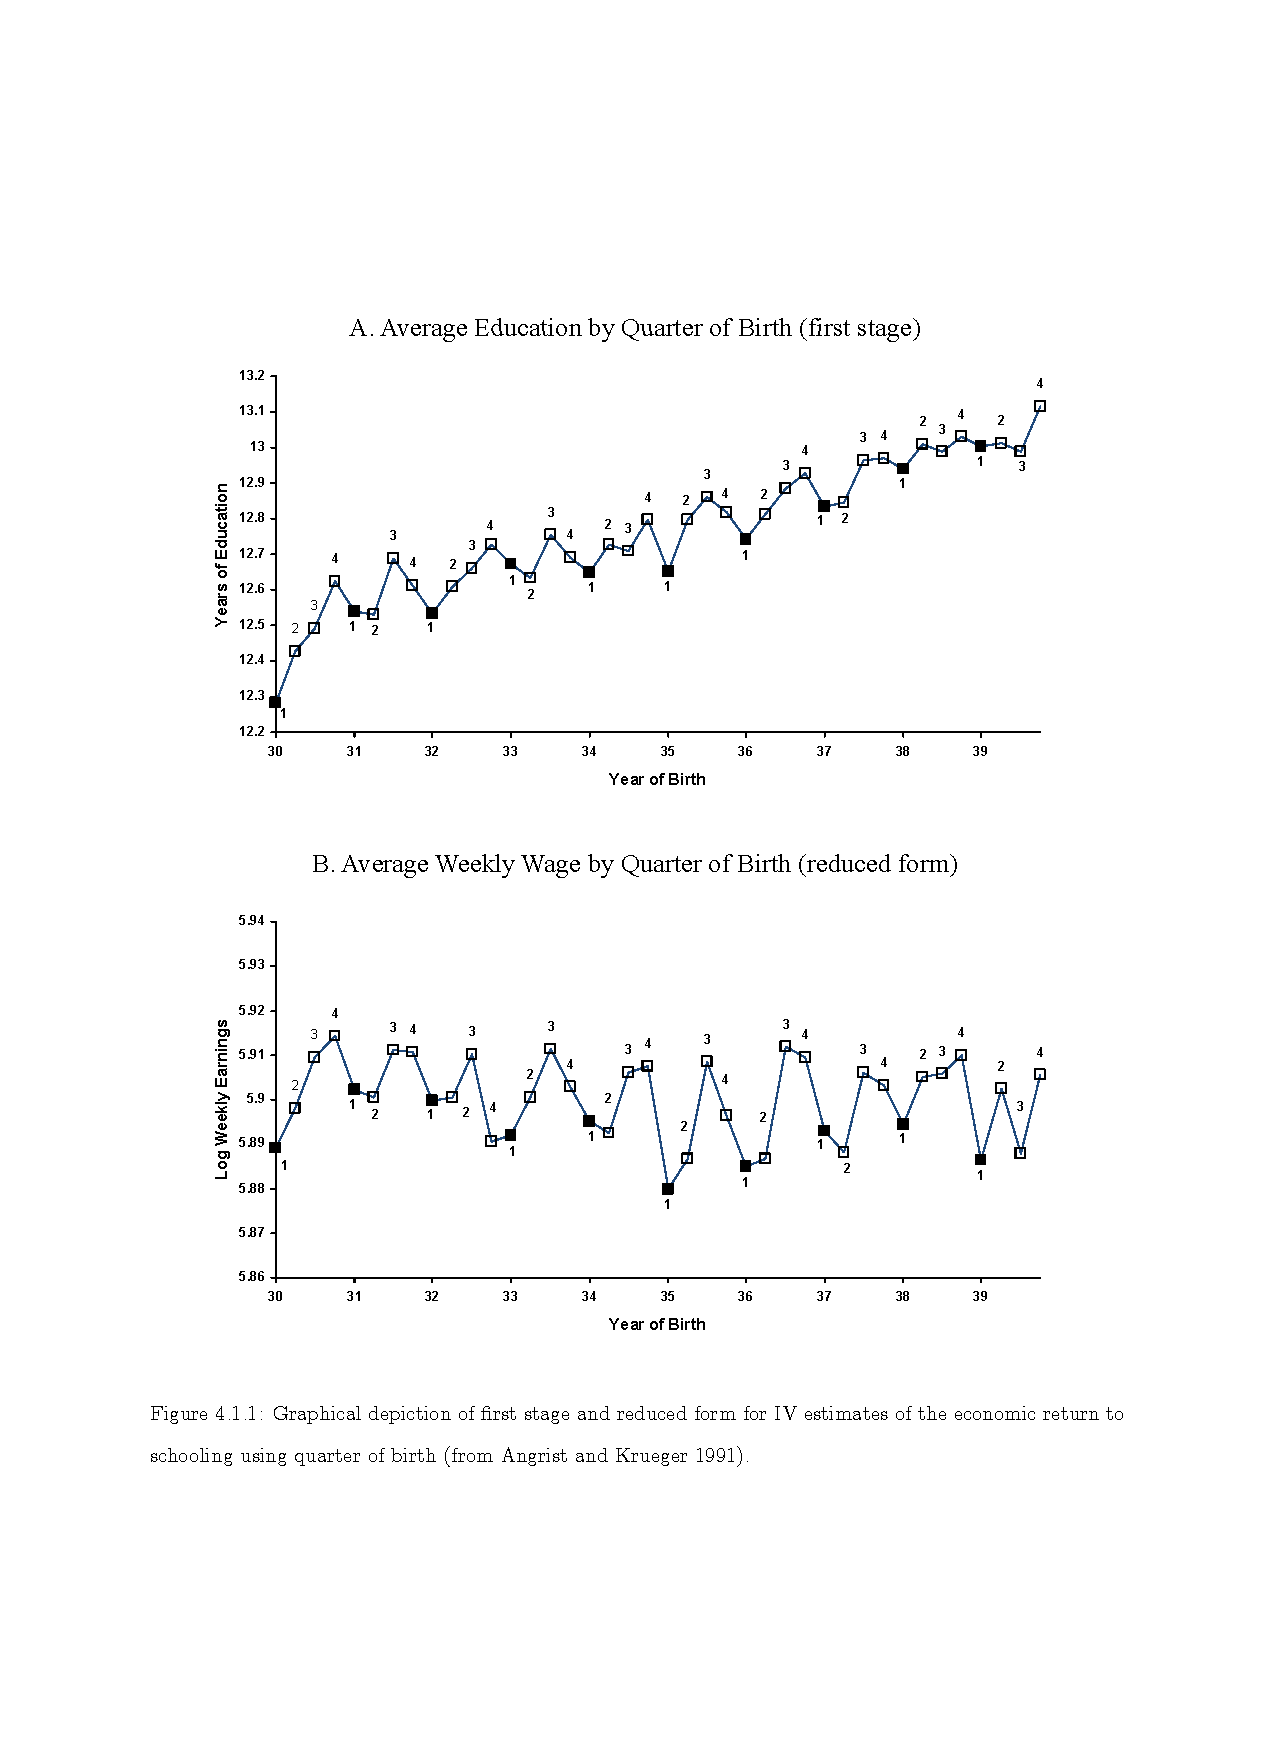
\includegraphics[width=0.7\linewidth]{graphs/ap_411.pdf}
\end{figure}
\end{center}
 }





\begin{frame}
\frametitle{Multiple Instruments}

\begin{itemize}
\item $z_{1i}, z_{2i} , z_{3i}$ dummy variables for quarter of birth
\item 2 stage least squares estimation
\item First stage equation
\[ \begin{array}{cl}
s_{i}= X_{i}^{'}\pi_{10}+\pi_{11}z_{1i}+\pi_{12}z_{2i}+\pi_{13}z_{3i}+\xi_{i1}
    \end{array}
\]

\item $\hat{s}_{i}$ fitted values from first stage regression

\item 2SLS "instrument": linear combination of all instrumental variables -- increases efficiency.
\end{itemize}

\end{frame}

 \frame{ \frametitle{}
\begin{center}
\begin{figure}[t]
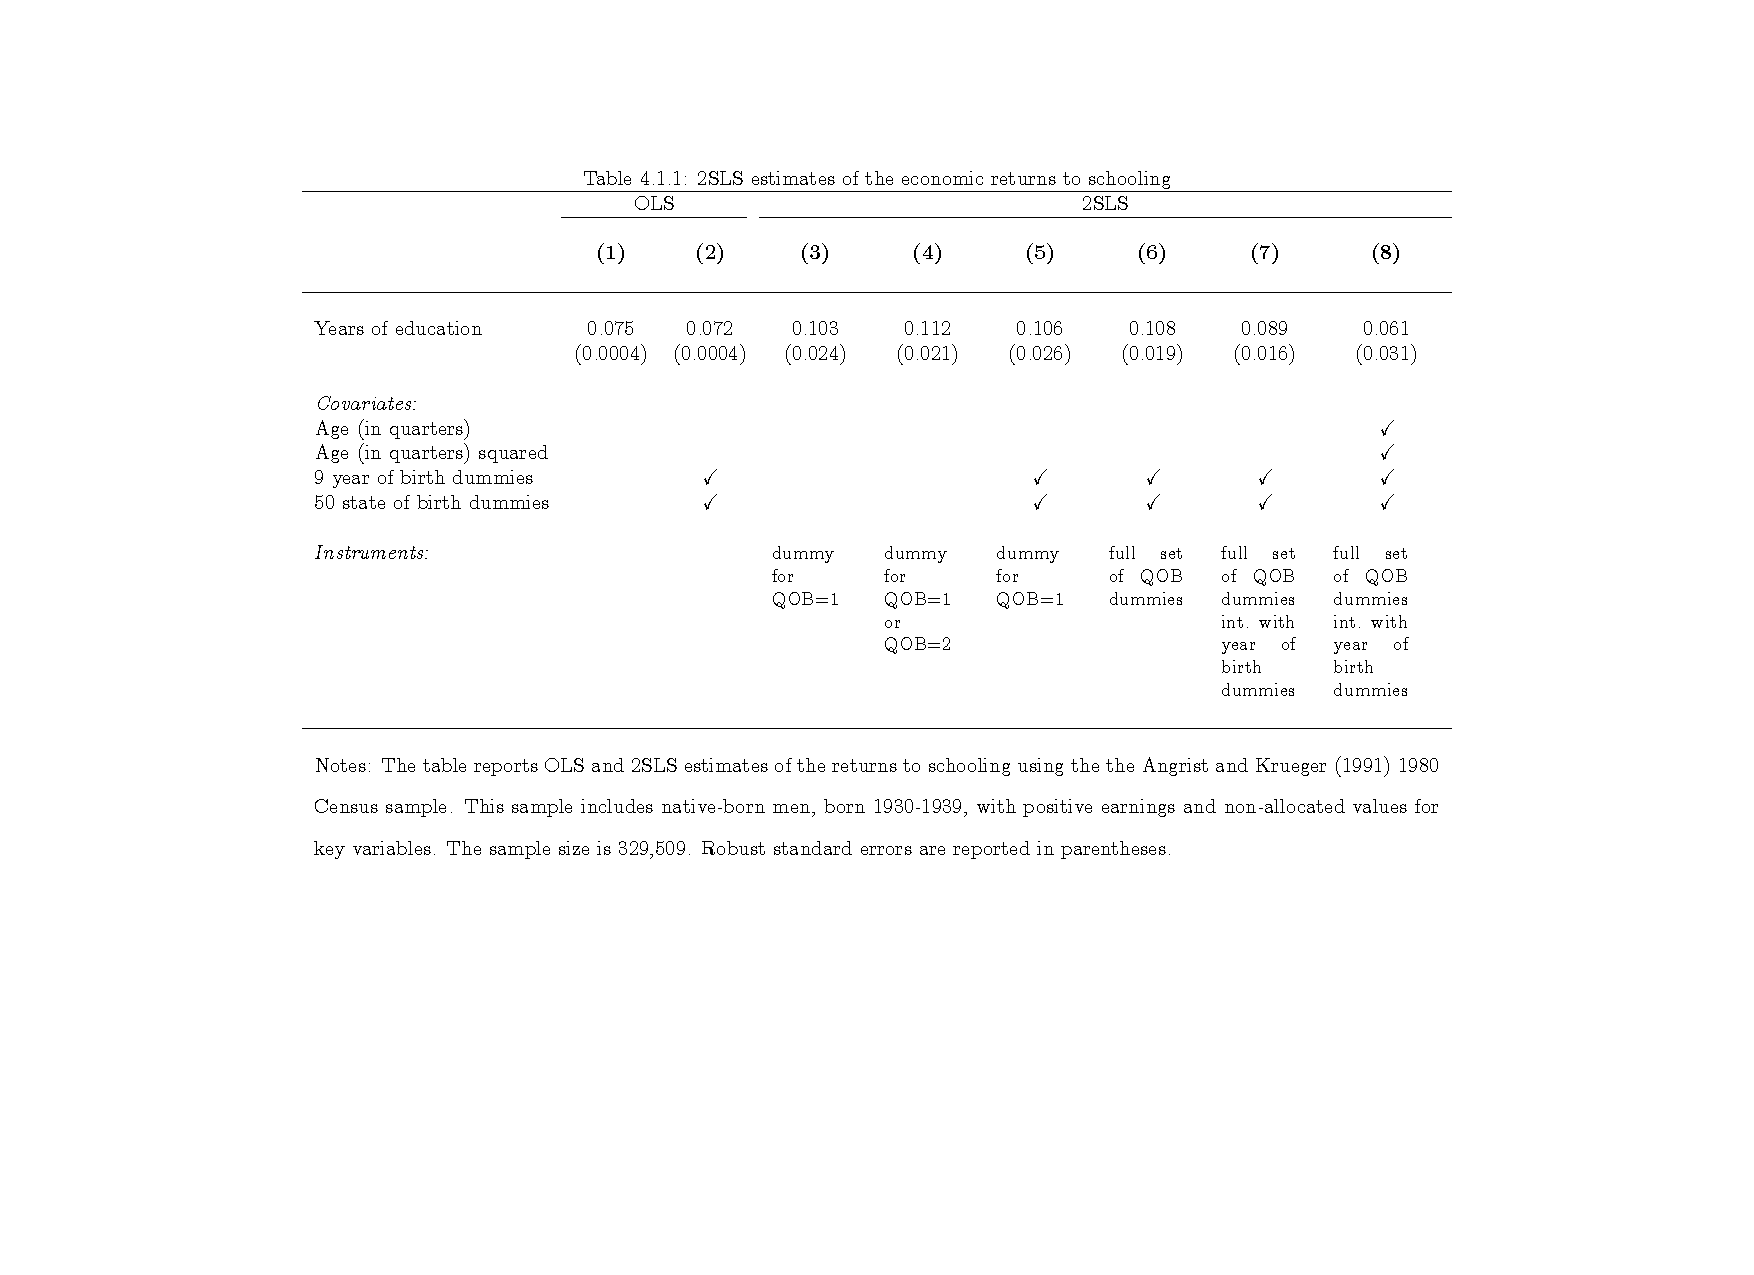
\includegraphics[width=1.1\linewidth]{graphs/ap_tab411.pdf}
\end{figure}
\end{center}
 }

% slide 14


\begin{frame}
\frametitle{Wald Estimator}
\begin{itemize}
\item Special case:  $z_{i}$ dummy variable
\item Structural model $Y_{i} = \alpha+ \rho s_{i}+ \eta_{i}$
\begin{eqnarray*}
 E(Y_i|z_i) &=&  \alpha + \rho E(s_i|z_i)  +  E(\eta_i|z_i) \\
 E(Y_i|z_i=1) &=&  \alpha  + \rho E(s_i|z_i=1) +  E(\eta_i|z_i=1) \\
 E(Y_i|z_i=0) &=&   \alpha  + \rho E(s_i|z_i=0)+  E(\eta_i|z_i=0) 
\end{eqnarray*}

\item Wald estimator
\begin{eqnarray*}
 \rho &=& \frac{E\left[Y_{i}|z_{i}=1\right]-E\left[Y_{i}|z_{i}=0\right]}{E\left[s_{i}|z_{i}=1\right]-E\left[s_{i}|z_{i}=0\right]} \\
 &=&\frac{\text{difference in mean earnings by z}}{\text {difference in mean schooling by z}}
\end{eqnarray*}

\end {itemize}
\end {frame}
%
%\begin{frame}
%\frametitle{Applications}
%
%\begin{itemize}
%\item Effects of veteran status on earnings
%	\begin{itemize}
%		\item Does serving in the military have an impact on earnings later in life?
%		\item Instrument: Vietnam war draft lottery  (Angrist,1990)
%	\end{itemize}
%\item Effects of family size on female labor supply (Angrist and Evans, 1998)
%	\begin{itemize}
%		\item Instrument: Multiple births, sex composition
%	\end{itemize}
%\item Returns to schooling
%	\begin{itemize}
%		\item Ability bias or sorting based on returns to schooling?
%		\item Instrument: Quarter of birth (Angrist and Krueger, 1991)
%		\item Instrument: Proximity to college (Card, 1993)
%	\end{itemize}
%
%\end{itemize}
%
%\end{frame}


\begin{frame}
\frametitle{Draft lottery}

\begin{itemize}
\item U.S. conscription during the Vietnam war era
	\begin{itemize}
		\item Institution of draft lottery in 1970
		\item each year 1970-1972 a random sequence of lottery numbers were assigned to each birth date in the cohort of 19-year olds.
		\item lottery numbers below a cutoff were eligible to be drafted
		\item exceptions for volunteers, school attendance, bad health etc.
	\end{itemize}
\item use draft eligibility status as binary instrument for military service
\item lottery number positively correlated with veteran status: relevance
\item lottery number uncorrelated to other determinants of earnings: exclusion restriction
\item discrete instrument: lottery number groups, visual IV
\end{itemize}

\end{frame}
\frame{ \frametitle{}
\begin{center}
\begin{figure}[t]
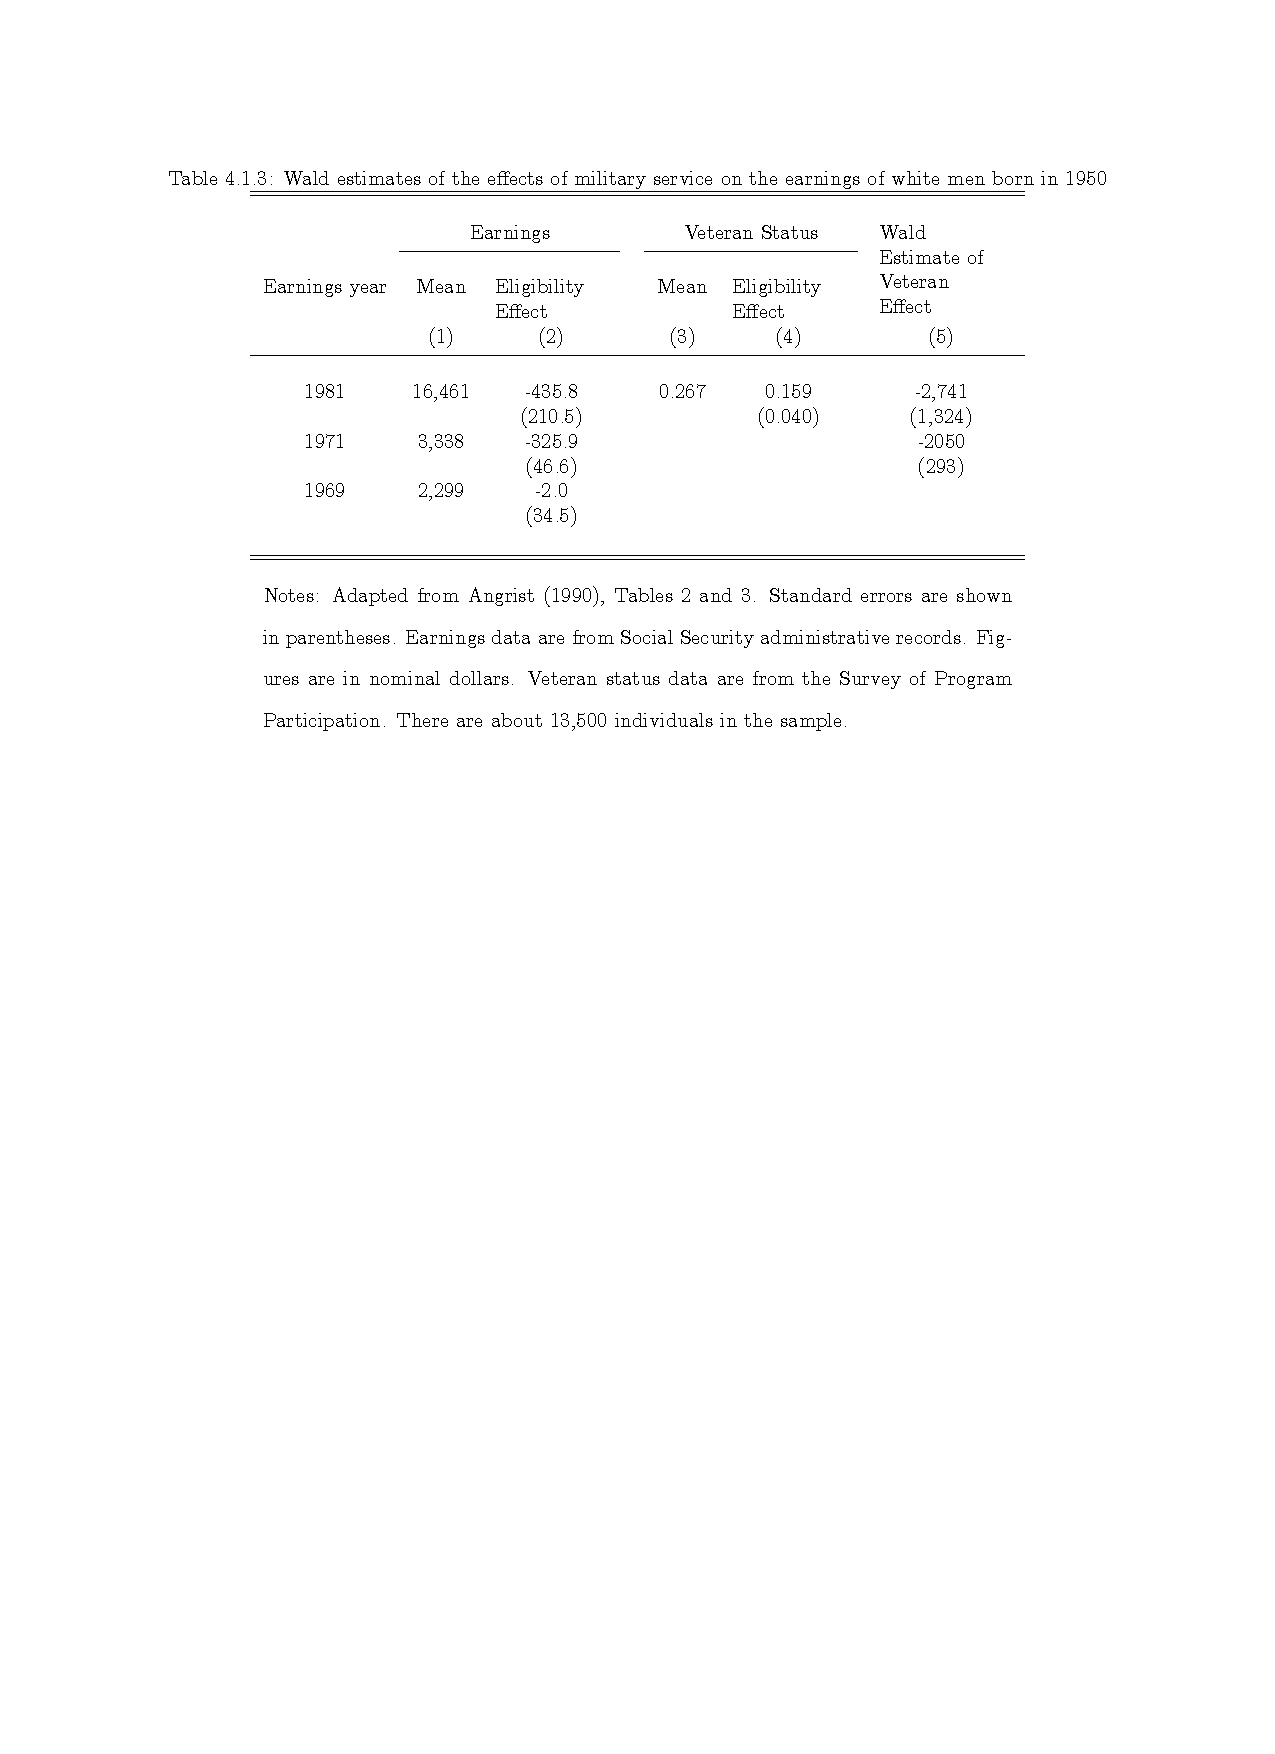
\includegraphics[width=1.0\linewidth]{graphs/ap_413.pdf}
\end{figure}
\end{center}
 }

 \frame{ \frametitle{}
\begin{center}
\begin{figure}[t]
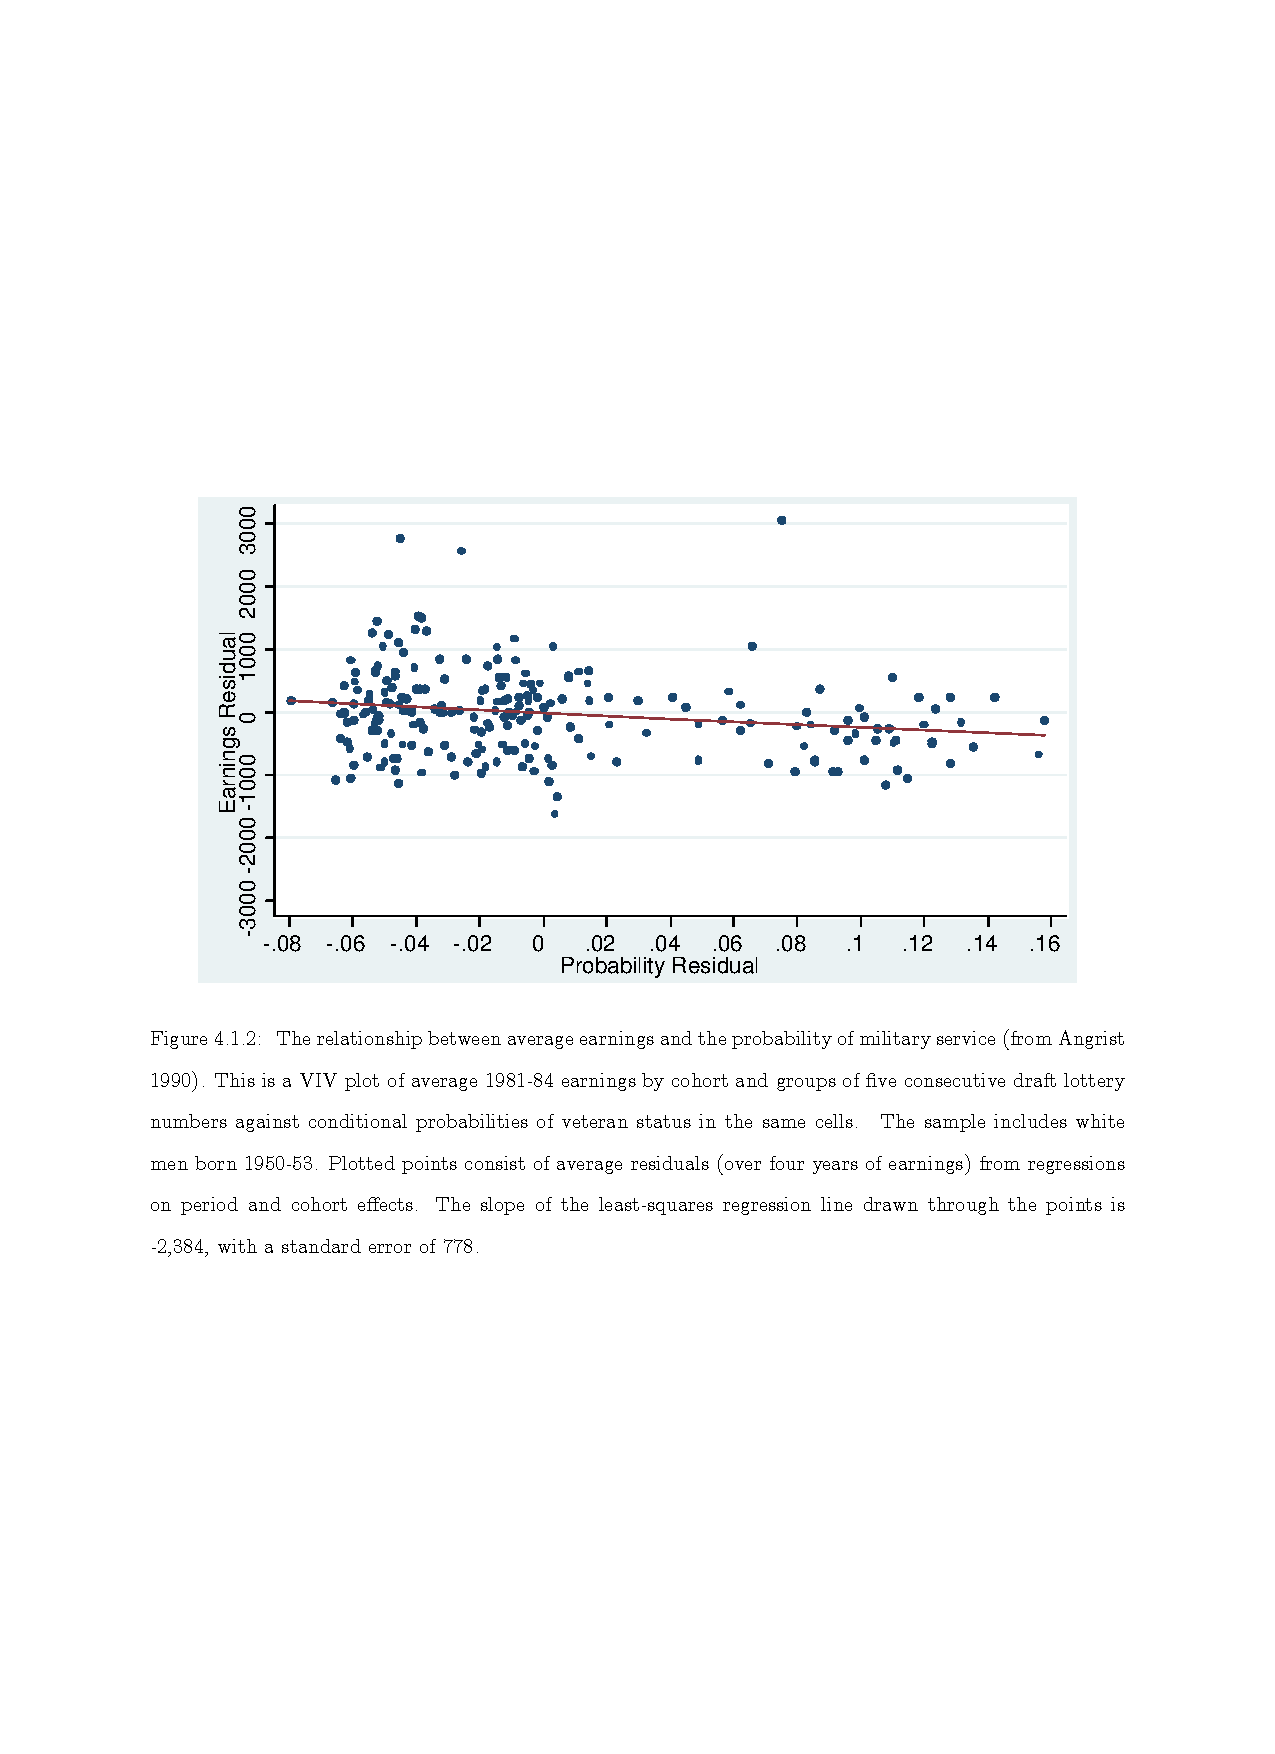
\includegraphics[width=1.0\linewidth]{graphs/ap_412.pdf}
\end{figure}
\end{center}
 }
\frame{ \frametitle{}
\begin{center}
\begin{figure}[t]
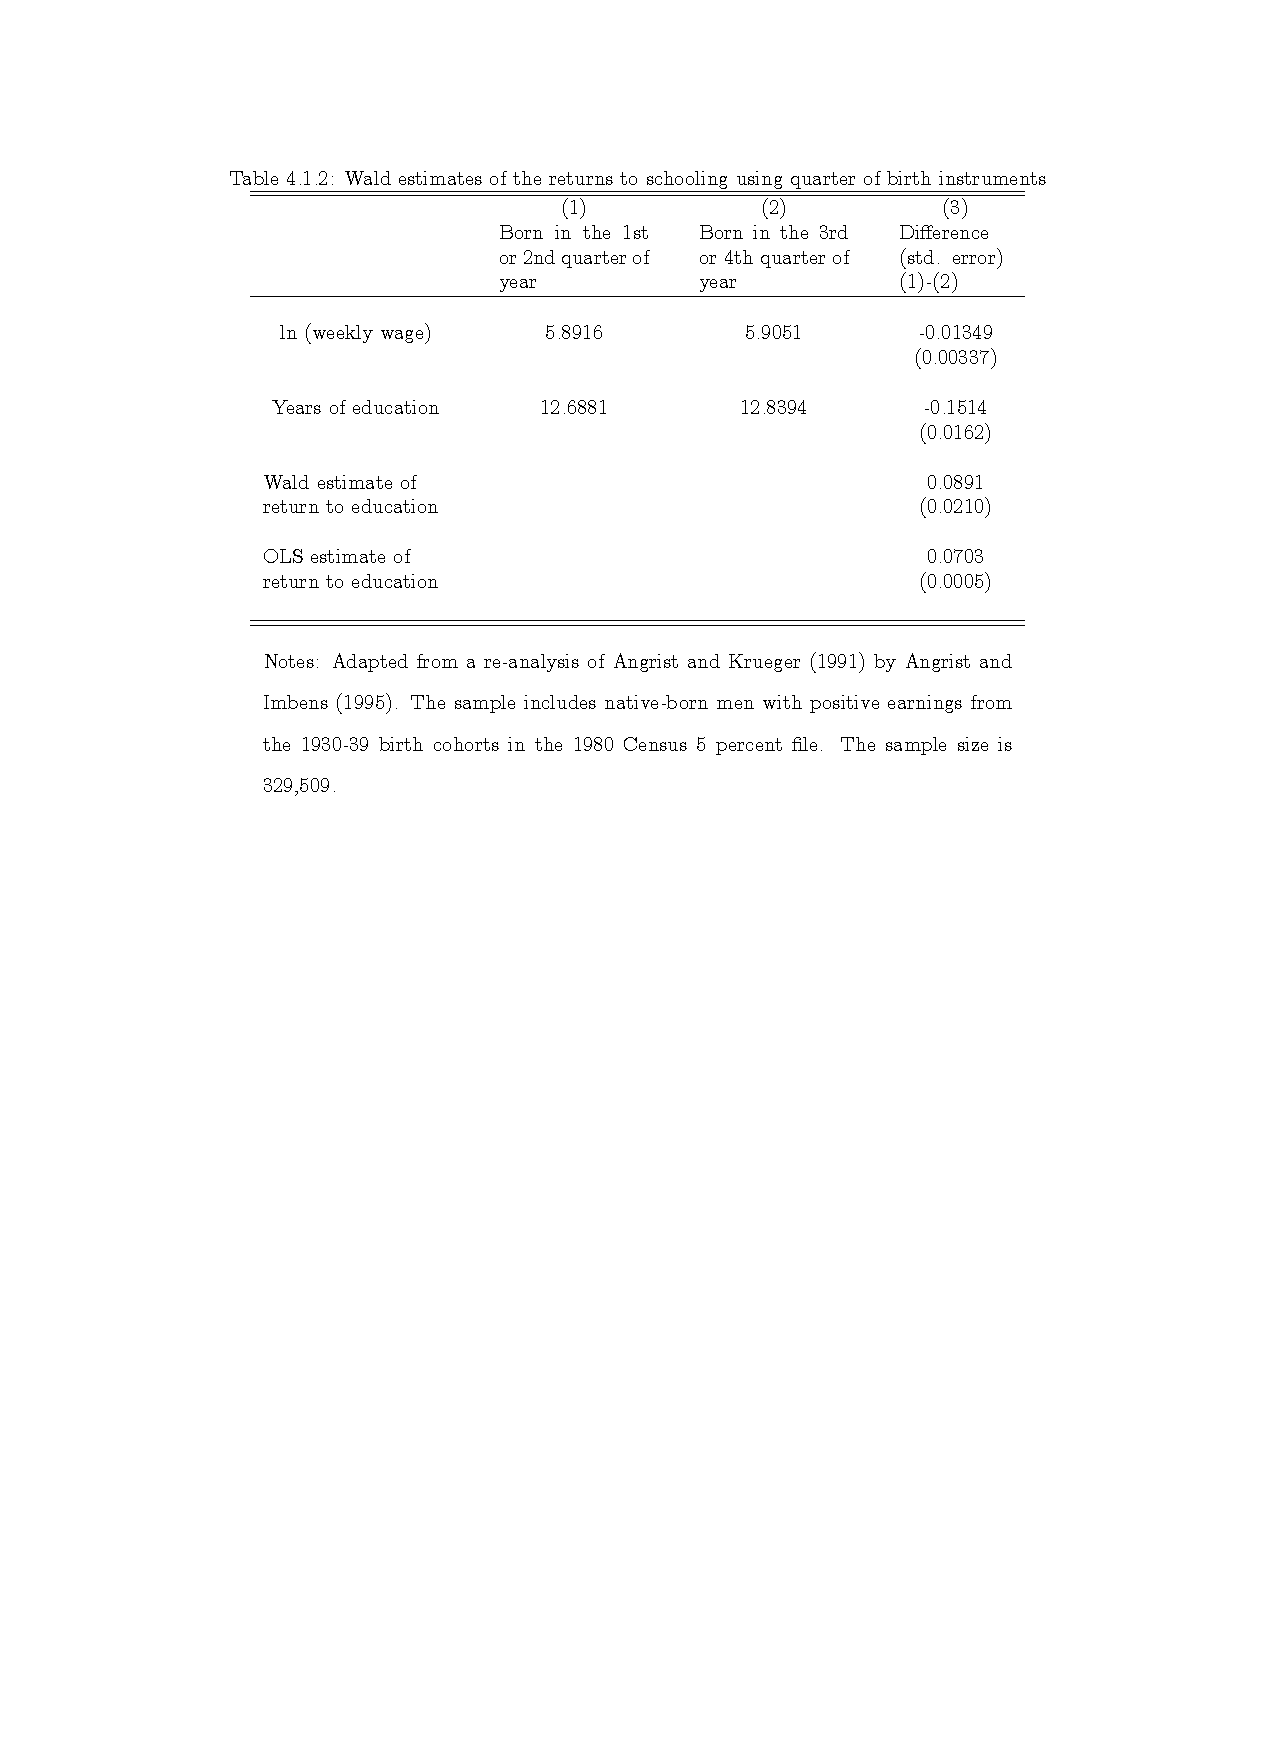
\includegraphics[width=1.0\linewidth]{graphs/ap_tab412.pdf}
\end{figure}
\end{center}
 }
 
 \begin{frame}
\frametitle{Family Size and Female Labor Supply}

\begin{itemize}
\item Women with more children work less
	\begin{itemize}
		\item Effect of family size?
		\item Selection?
	\end{itemize}
\item Instrumental variables which exogenously increase family size
\item Multiple births 
\item Sex composition
\end{itemize}

\end{frame}

 \frame{ \frametitle{}
\begin{center}
\begin{figure}[t]
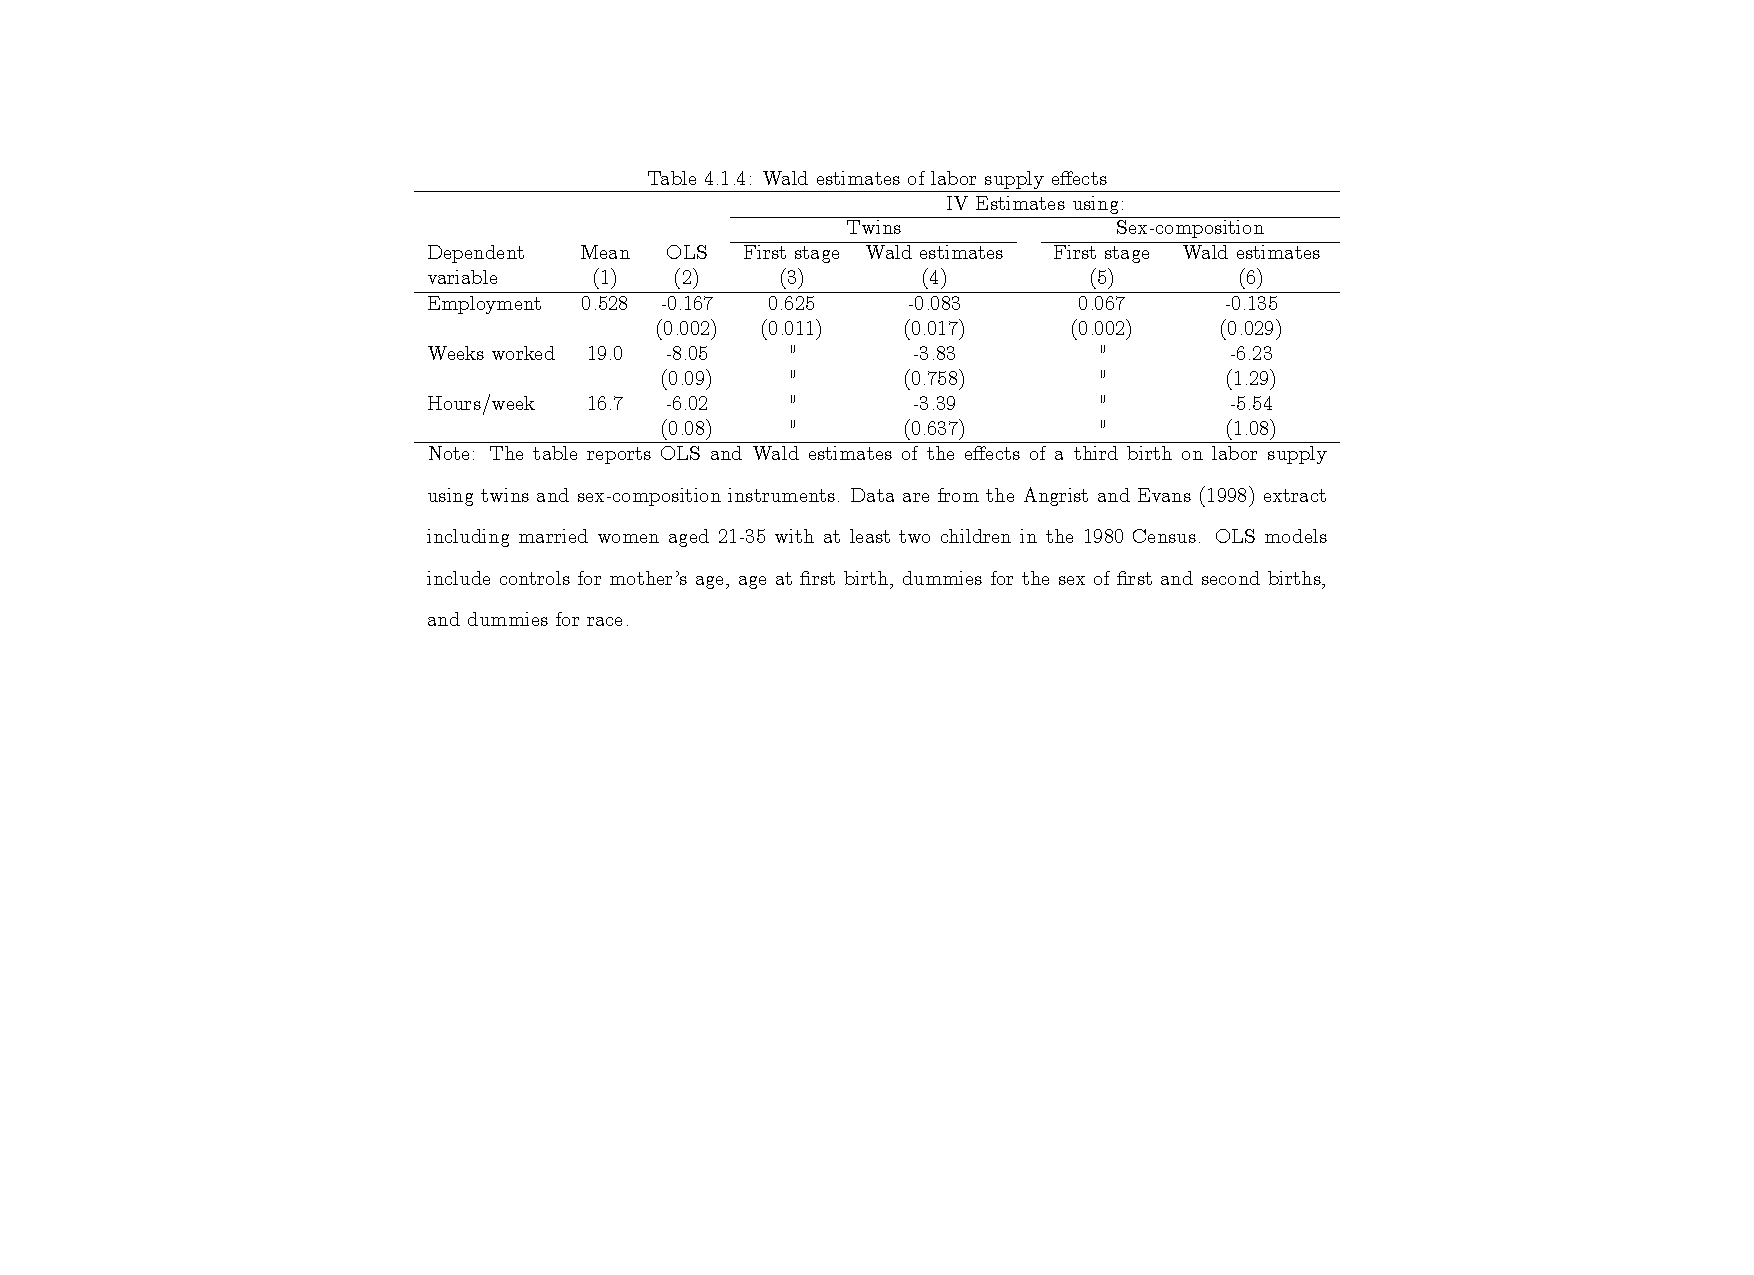
\includegraphics[width=1.0\linewidth]{graphs/ap_tab414.pdf}
\end{figure}
\end{center}
 }





\begin{frame}
\frametitle{College Proximity}
\begin{itemize}
\item "Using geographic variation in college proximity to estimate the return to education'', Card (1993, NBER WP 4483)
\end{itemize}
\end{frame}


\begin{frame}
\frametitle{Data}

\begin{itemize}
\item National Longitudinal Survey of Youths
\item Young men age 14-24 in 1966
\item 1st survey 1966
	\begin{itemize}
      \item family composition
       \item father's, mother's education
       \item characteristics of local labor market e.g. college
      \end{itemize}
\item Follow up surveys every 2 years
	\begin{itemize}
      \item large attrition 20\% drop out in first 3 years
       \item select 1976 interview for labor market information
       \item education, wages
      \end{itemize}
      \end{itemize}

\end{frame}


\frame{ \frametitle{}
\begin{center}
\begin{figure}[t]
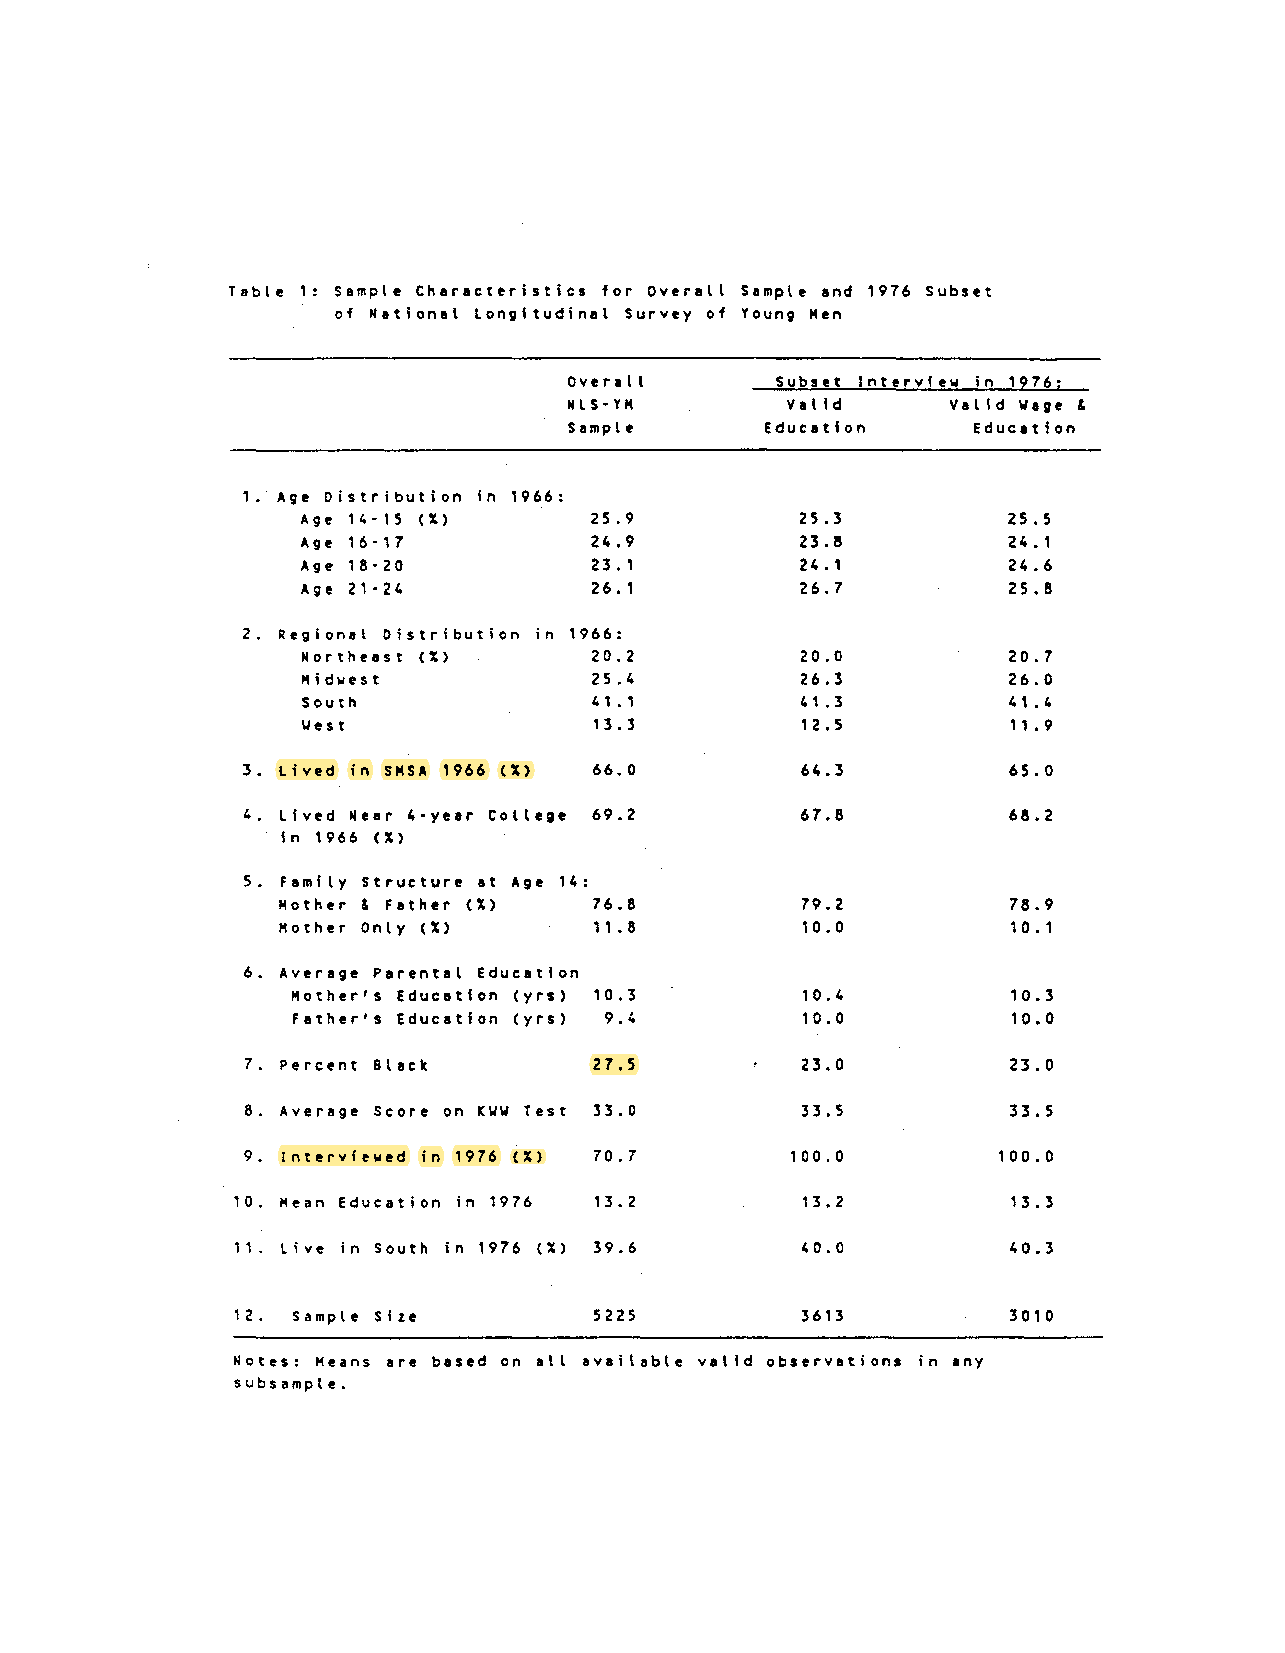
\includegraphics[width=0.7\linewidth]{graphs/card_tab1.pdf}
\end{figure}
\end{center}
 }
 
 
 
 \begin{frame}
\begin{itemize}
\item Linear model

\begin{eqnarray*}
           Y_{i}= \alpha+ \rho s_{i}+ \eta_{i}
      \end{eqnarray*}
      \end{itemize}
\end{frame}



 \frame{ \frametitle{}
\begin{center}
\begin{figure}[t]
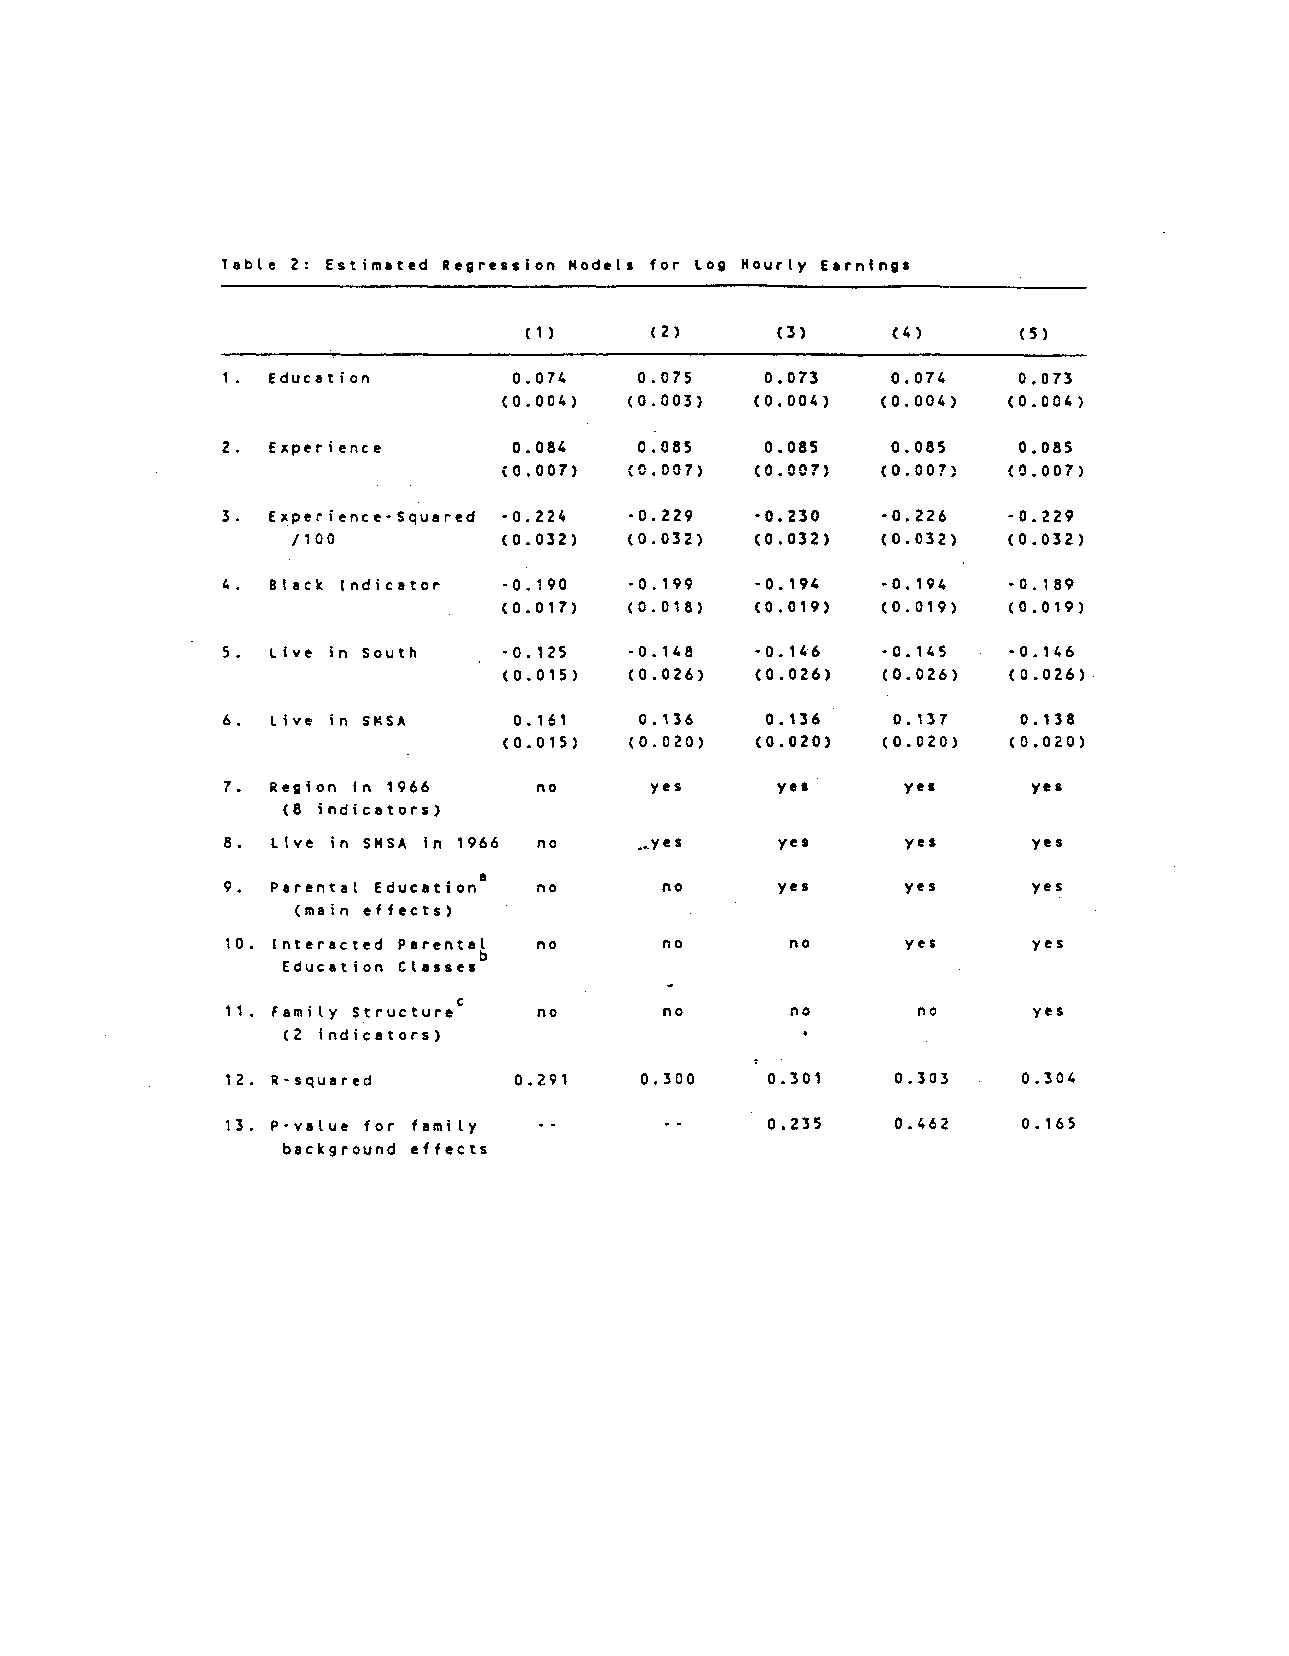
\includegraphics[width=0.9\linewidth]{graphs/card_tab2.pdf}
\end{figure}
\end{center}
 }

 
 \begin{frame}
 \begin{itemize}

\item Ability Bias
      \begin{itemize}
      \item Individual with high test scores have higher schooling upward biased OLS $\hat{\rho}$
      \end{itemize}

\item Absence of "pure" random assignment
     \begin{itemize}
      \item Use the presence of a nearby college as exogenous variation in education
      \item Students who grow up in an area without a college face a higher cost of college education, since the option of living at home is precluded.
      \end{itemize}
            \begin{itemize}
      \item  ${\rho}$ might depend on levels of income
      \end{itemize}
\end{itemize}
\end{frame}


\frame{ \frametitle{Relevance}
\begin{center}
\begin{figure}[t]
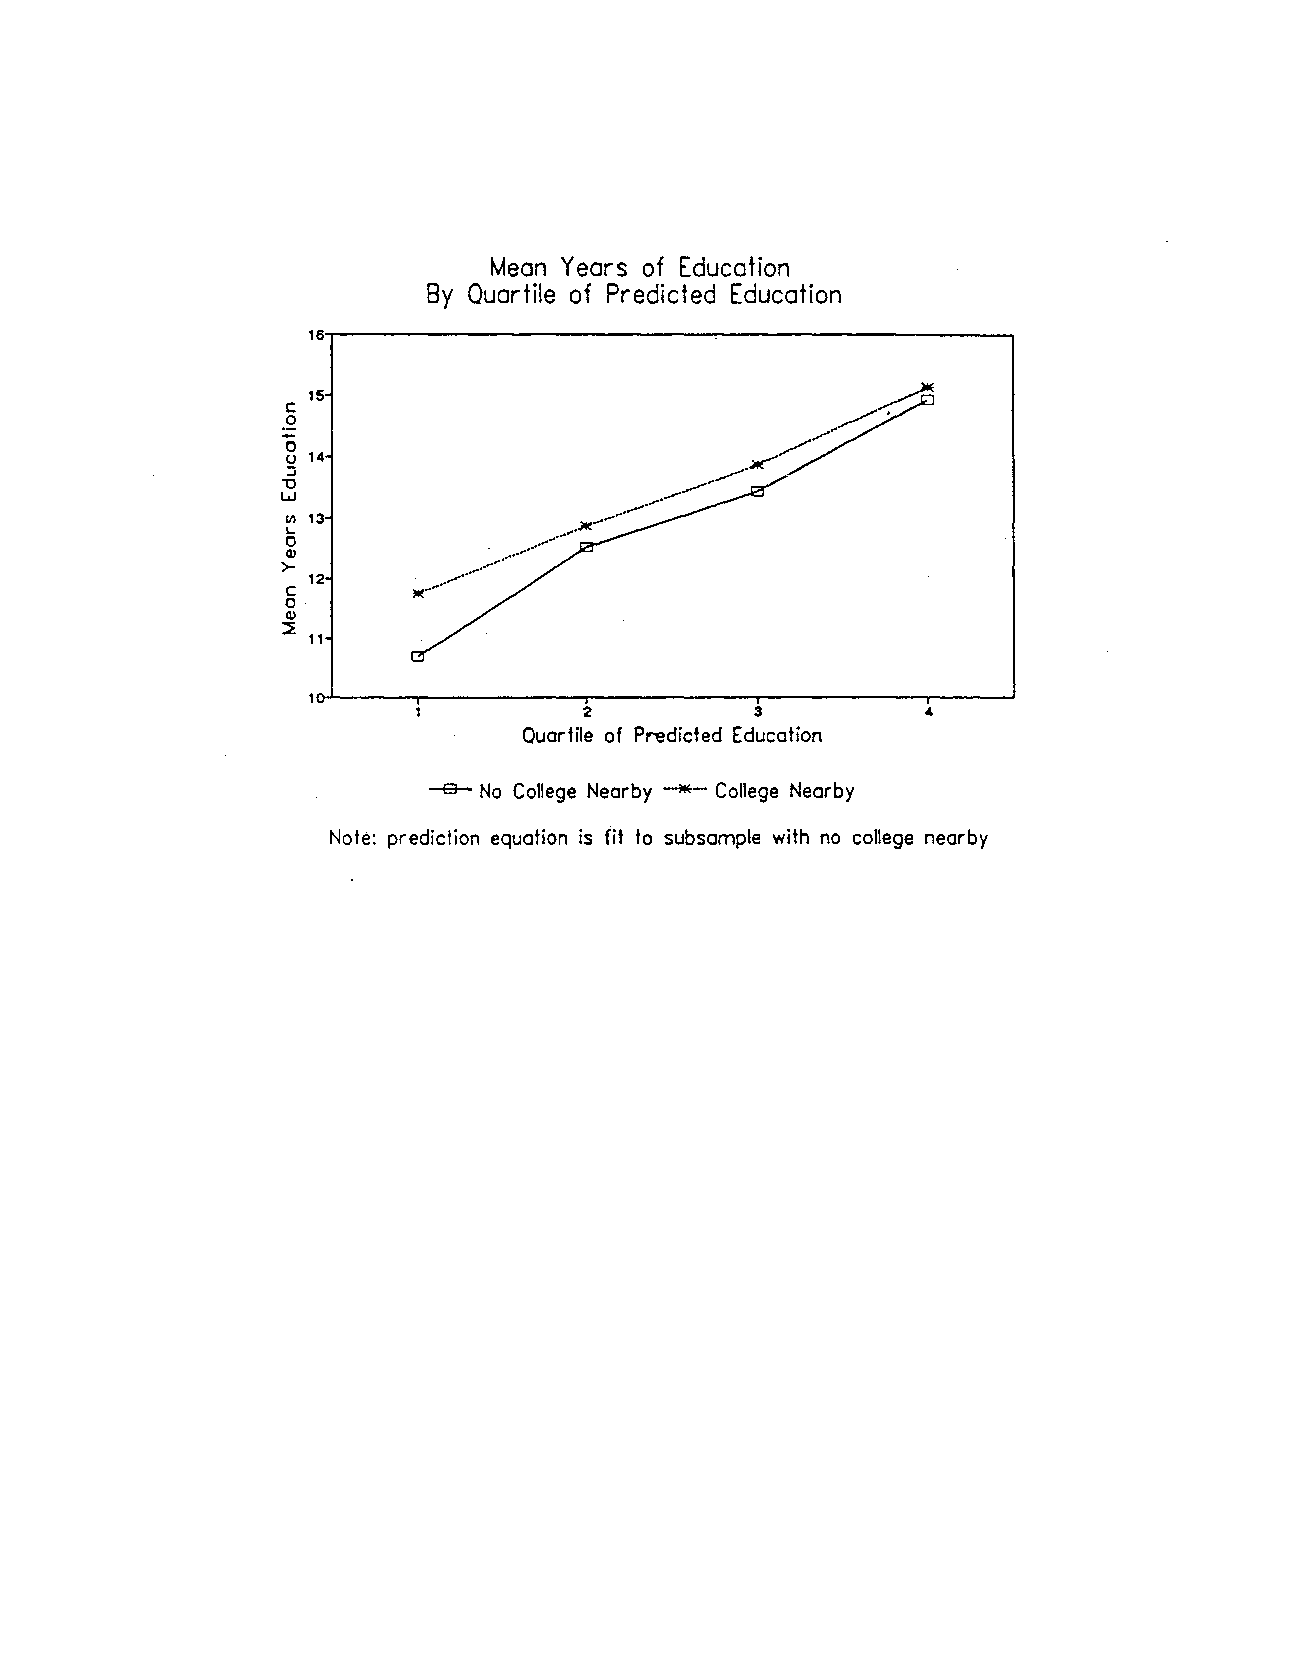
\includegraphics[width=1.0\linewidth]{graphs/card_fig1.pdf}
\end{figure}
\end{center}
 }




\begin{frame}
\frametitle{Structural Model Equation}

Model
\begin{eqnarray*}
  Y_i &=& \alpha + \rho s_i + \gamma_1 exper_i + \gamma_2 exper_i^2 + \eta_i 
\end{eqnarray*}
\begin{itemize}
\item Potential experience $exper_i = age_i - s_i -6$
\item Additional covariates: parents' education, region of residence, etc
\item Proxy for ability: `knowledge of the world of work' test score
\item instrument $c_i$ college proximity
\item First stage
\begin{eqnarray*}
  s_i &=& \pi_{10} + \pi_{11} c_i  + \pi_{12} exper_i + \pi_{13} exper_i^2 + \xi_{1i}
\end{eqnarray*}
\end{itemize}

\end{frame}






 \frame{ \frametitle{}
\begin{center}
\begin{figure}[t]
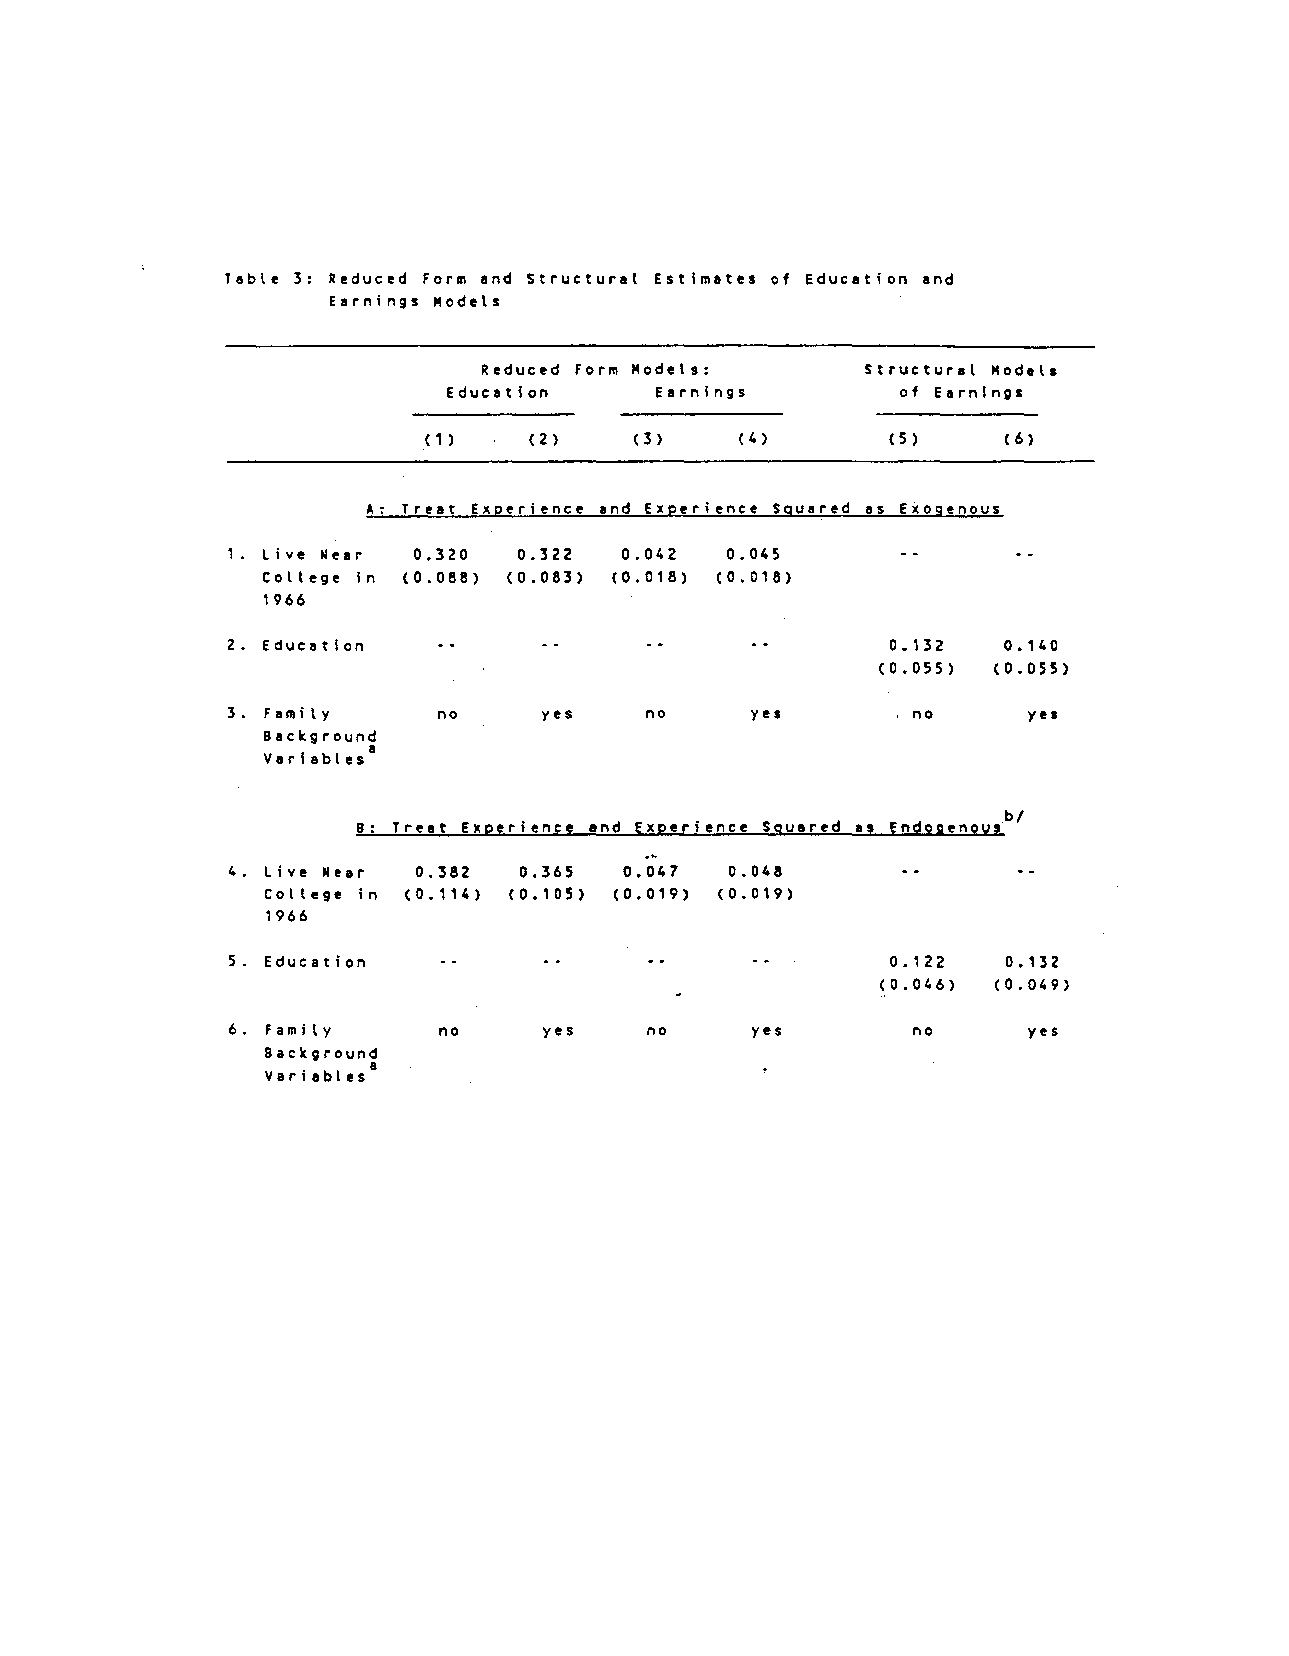
\includegraphics[width=1.0\linewidth]{graphs/card_tab3.pdf}
\end{figure}
\end{center}
 }


\begin{frame}
\frametitle{Multiple Endogenous Variables}
\begin{itemize}
\item  $experience$, $experience^{2}$
\item  Need two additional excluded variables $z_{2}$, $z_{3}$ correlated with $experience$, $experience^{2}$
\item $age$, $age^{2}$
\item \textbf{Three} first stage equations:
\begin{eqnarray*}
s_i &=& X_{i}^{'}\pi_{10}+\pi_{11}z_{1i}+\pi_{12}z_{2i}+\pi_{13}z_{3i}+\xi_{1i}\\
exper_i &=& X_{i}^{'}\pi_{20}+\pi_{21}z_{1i}+\pi_{22}z_{2i}+\pi_{23}z_{3i}+\xi_{2i}\\
exper_i^{2} &=&  X_{i}^{'}\pi_{30}+\pi_{31}z_{1i}+\pi_{32}z_{2i}+\pi_{33}z_{3i}+\xi_{3i}
\end{eqnarray*}

\item Reduced form equation:
\begin{eqnarray*}
Y_i &=& X_{i}^{'}\pi_{40}+\pi_{41}z_{1i}+\pi_{42}z_{2i}+\pi_{43}z_{3i}+\xi_{4i}\\
\end{eqnarray*}
\end{itemize}
\end{frame}







  \frame{ \frametitle{}
\begin{center}
\begin{figure}[t]
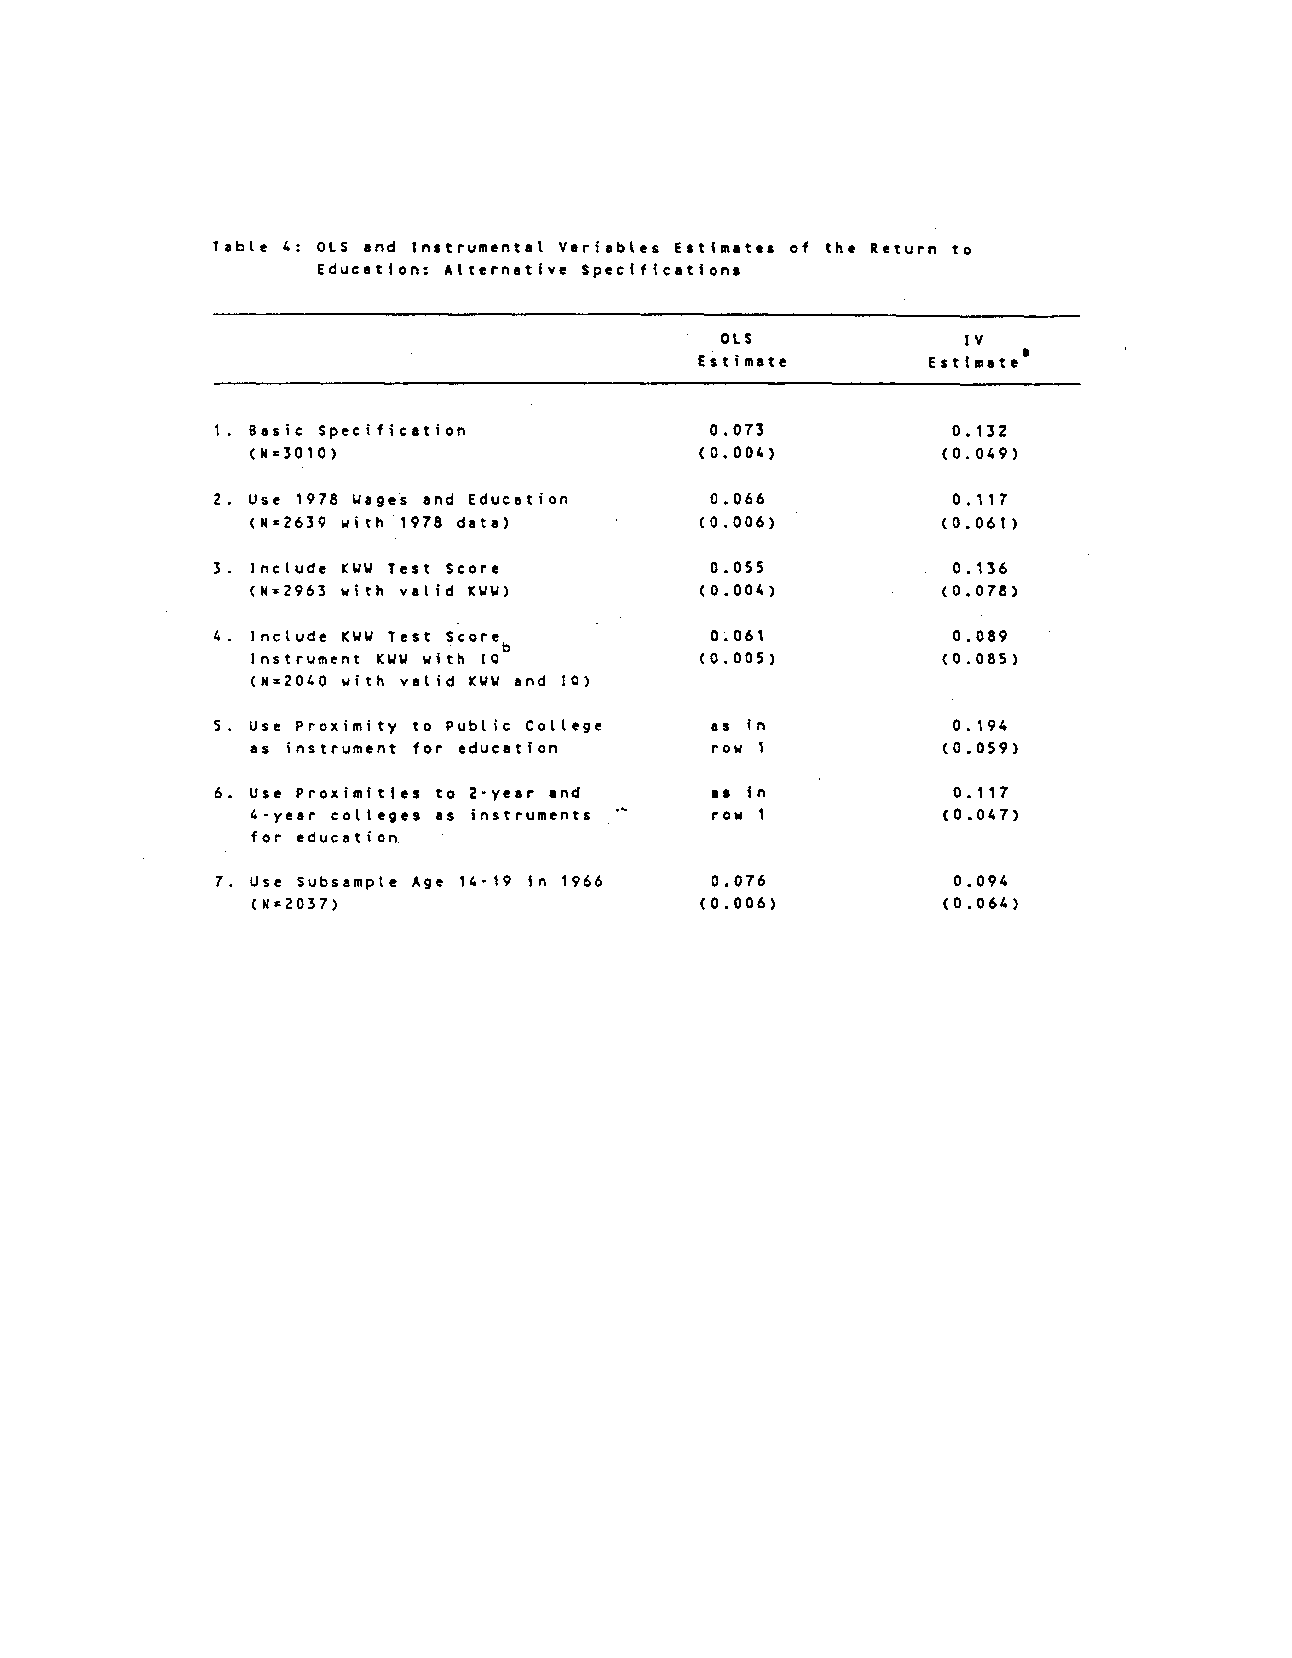
\includegraphics[width=1.0\linewidth]{graphs/card_tab4.pdf}
\end{figure}
\end{center}
 }
 
 
\begin{frame}
\frametitle{Multiple Instruments}

\begin{itemize}
\item $z_{1i}$ proximity to 4 year college
\item $z_{2i}$ proximity to 2 year college

\[ \begin{array}{cl}
s_{i}= X_{i}^{'}\pi_{10}+\pi_{11}z_{1i}+\pi_{12}z_{2i}+\xi_{i1}
    \end{array}
\]

\item $\hat{s}_{i}$ fitted values from first stage regression

\item 2SLS "instrument": Residual from a regression of first stage fitted values on exogenous covariates increases efficiency.
\end{itemize}

\end{frame}
 
\begin{frame}
\frametitle{Exclusion restriction}
\begin{itemize}
\item Exclusion restriction does not allow for a \emph{direct} effect of college proximity on earnings.
\begin{itemize}
  \item Better schools in college areas
  \item Geographic wage premia
  \item Selection of families into college areas
\end{itemize}
\end{itemize}

\end{frame}


\begin{frame}
\frametitle{Direct effect from college proximity}

\begin{itemize}

\item Idea: college proximity should have a bigger effect on educational choice of low income families 
\item Instrument for education: $c_i * p_i$ were $p_i$ is an indicator for low parental background
\item First stage
\begin{eqnarray*}
  s_i &=& \pi_{10} + \pi_{11} c_i + \pi_{12} (c_i* p_i) + \pi_{13} exper_i + \pi_{14} exper_i^2 + \xi_{1i}
\end{eqnarray*}
\item Earnings Equation
\begin{eqnarray*}
  Y_i &=& \alpha + \delta c_i + \rho s_i + \gamma_1 exper_i + \gamma_2 exper_i^2 + \eta_i
\end{eqnarray*}

\end{itemize}

\end{frame}

  \frame{ \frametitle{}
\begin{center}
\begin{figure}[t]
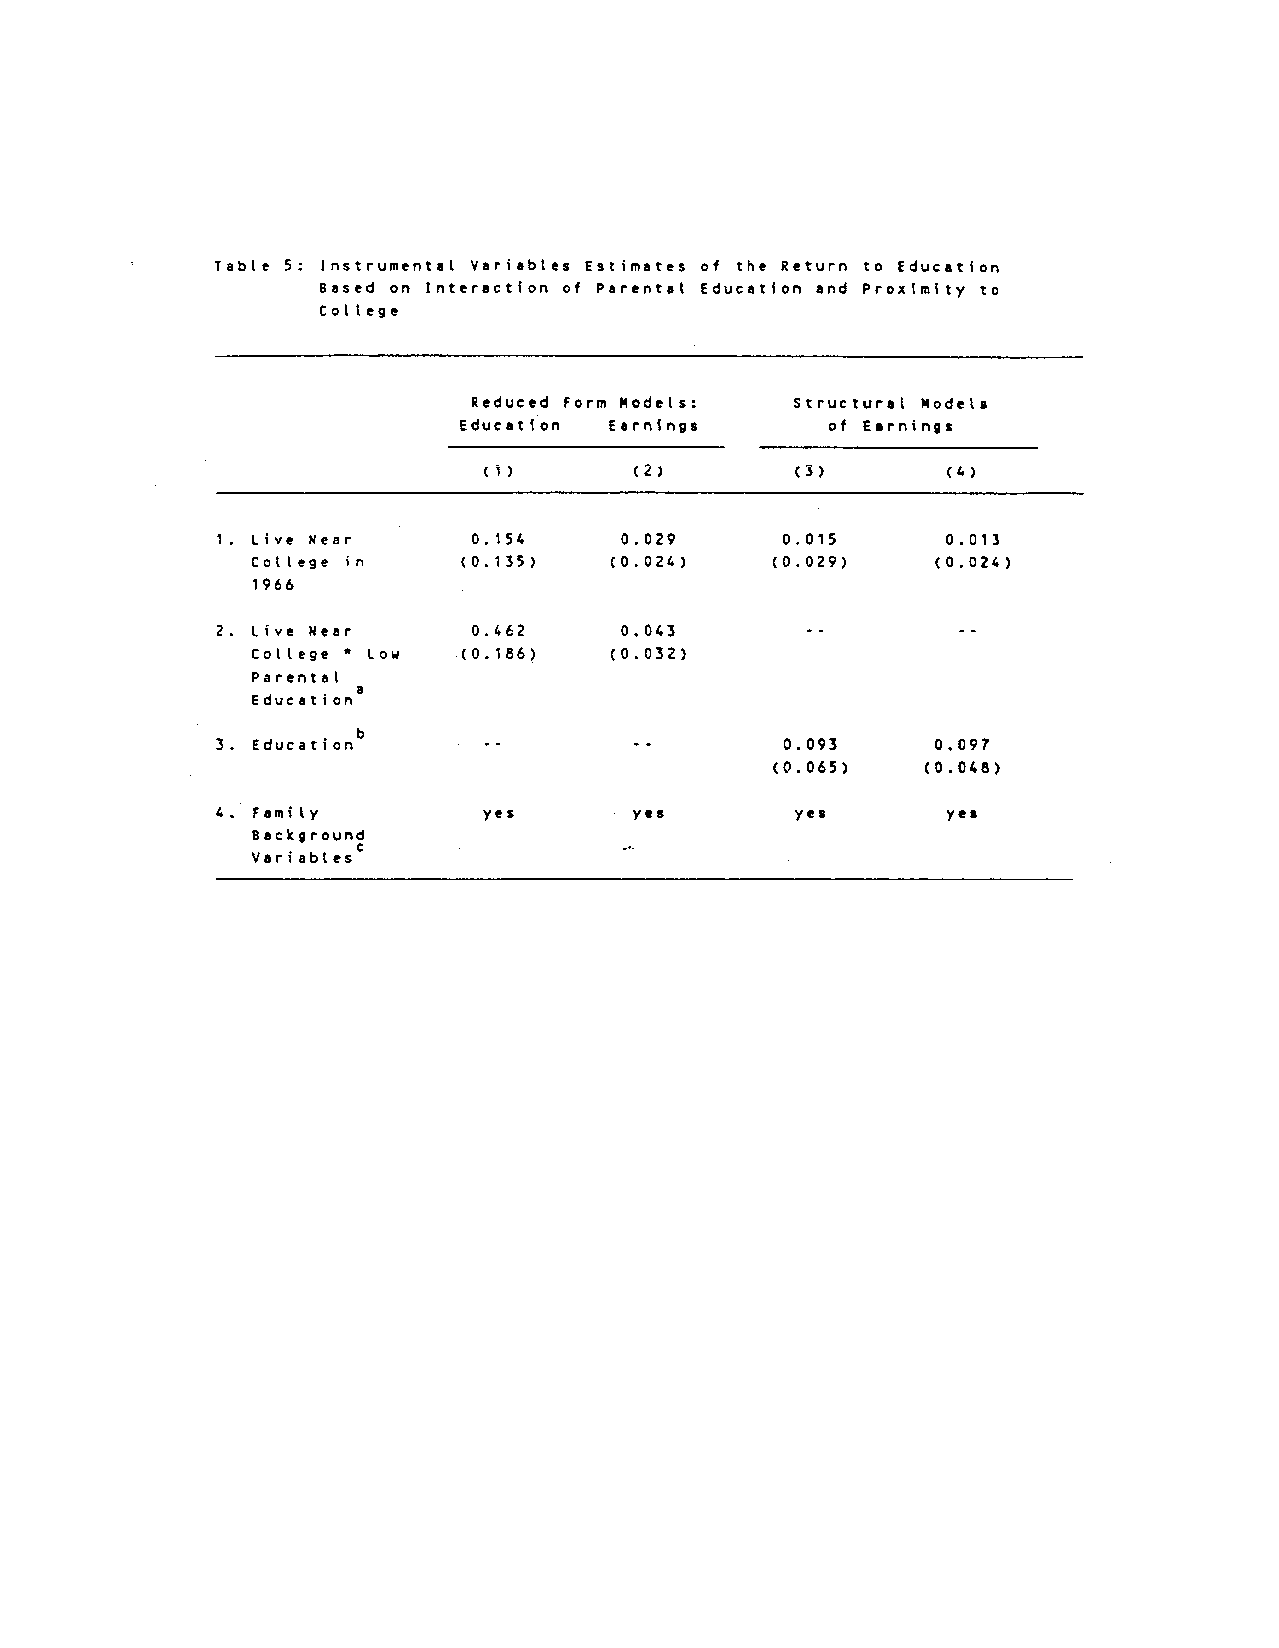
\includegraphics[width=1.0\linewidth]{graphs/card_tab5.pdf}
\end{figure}
\end{center}
 }





%slide 20

\begin{frame}
\frametitle{Testing for Endogeneity}
\begin{itemize}
\item 2SLS less efficient than linear regression (larger standard errors)

\begin{eqnarray*}
   Y_{i} &=& \alpha X_{i}^{'}+ \rho s_{i}+ \eta_{i}
\end{eqnarray*}

\item $z_{i}$ exogenous instrument.
\item If $Cov\left(s_{i}, \eta_{i}\right)=0$, we can use linear regression
    \begin {itemize}
    \item 2SLS consistent but less efficient
  \end {itemize}
\item If $Cov\left(s_{i}, \eta_{i}\right)\neq0$, should use 2SLS with instrument $z_{i}$

\item Idea: Compare OLS and 2SLS estimates


\end{itemize}

\end{frame}



%slide 21

\begin{frame}
\frametitle{Testing for Endogenity}
\begin{itemize}
      \item First Stage
       \begin{eqnarray*}
           s_{i} &=& X_{i}^{'}\pi_{10}+ \pi_{11}z_{i}+ \xi_{1i}
      \end{eqnarray*}

      \item $Cov\left(s_{i}, \xi_{1i}\right)=0$


     \begin {itemize}
     \item Predict first stage residual $\hat{\xi}_{1i}$ and include it in structural equation.
    \end {itemize}

\begin{eqnarray*}
           Y_{i}= X_{i}^{'}\alpha+ \rho s_{i}+ \delta\hat{\xi}_{1i}+ error
      \end{eqnarray*}
\item Hausman Test:
     \item Test whether $\delta=0$

\begin{eqnarray*}
H_{0}: \delta=0
\end{eqnarray*}



\end{itemize}

\end{frame}




% slide 22
\begin{frame}
\frametitle{Testing Overidentification Restrictions}

\begin{eqnarray*}
           Y_{i}= X_{i}^{'}\alpha+ \rho s_{i}+ \eta_{i}
      \end{eqnarray*}
\begin{itemize}
\item Two instruments $z_{1}$ and $z_{2}$
\item We could generate 2 IV estimators one using $z_{1}$, one using $z_{2}$ and compare or check for correlation between IV-residuals with the other instrument.
\item Test procedure

     \begin{itemize}
       \item Estimate 2SLS using $z_{1}$ and $z_{2}$ and predict residuals $\hat{\eta}_{i}$
       \item Regress $\hat{\eta}_{i}$ on all exogenous variables and obtain $R^{2}$
       \item $H_{0}:$ $z_{1}$ and $z_{2}$ uncorrelated to $\eta_i$
       \item $nR^{2}\approx\chi^{2}_{q}$, $q=2$, number of instrument
\end{itemize}
\end{itemize}

\end{frame}



\begin{frame}
\frametitle{Testing Overidentification Restrictions}
\begin{itemize}
\item Caveat:
      \begin{itemize}
      \item IV estimators often imprecise tests don't have much power.
      \item Treatment effect heterogeneity
      \end{itemize}


\end{itemize}
\end{frame}


%------------------------------------------------------------------%
\begin{comment}

\begin{frame}
\frametitle{IV with heterogeneous treatment effects }
\begin{itemize}
\item The constant-effects assumption perhaps a bit unrealistic
\item Allow for the fact that some
men may have benefited from military service while others were undoubtedly hurt by it
\item The  IV methods fail to capture either ATE or ATT in a model with
heterogeneous treatment effects
\item This is because only a subset of the population is
affected by any particular instrumental variable
\item Under reasonably general assumptions, IV methods can be relied on to capture the effect of treatment on compliers (LATE)

\end{itemize}
\end{frame}


\begin{frame}
\frametitle{IV with heterogeneous treatment effects }

      \begin{itemize}
      \item Conditional independence, that is, that the
joint distribution of  $\left(Y_{1i}, Y_{0i}, D_{1i}, D_{0i} \right) \amalg Z_i $
      \item  monotonicity, which requires
that either $D_{1i} \geq D_{0i}$ for all $i$ or vice versa
      \end{itemize}

\end{frame}
\end{comment}

\end {document}






